\chapter{Results}\label{chap:results}
We estimate the single-breed model proposed in Equation~\ref{eq:single_breed_model}. The applied estimation engine is \textit{gamm4j} which we introduced in Section~\ref{sec:gammJ}. For each breed, data is subsampled from our dataset presented in Table~\ref{table:dataset_statistics}. The subsamples are generated by picking all samples from randomly selected farms until a sample threshold $t_s$ is reached. $t_s$ is determined by our available computational capacities. This resource limitation is discussed in Section~\ref{sec:cholesky_scalable}. We deliberately select all available samples from each randomly chosen farm in order for the model to implicitly incorporate the structural characteristics of the dairy farm and cow herd. Initially, we conduct the analysis on subsamples spanning the entire study period which is our primary focus. Then, we divide the data into two distinct periods, prior to and subsequent to 2010 and briefly describe the results in Section~\ref{sec:split_period}. This data split is justified by previous work from \cite{gisbert-queral_climate_2021} and also motivated by potential changes in the cows' thermoregulatory mechanisms due to breeding, or the abolition of milk quotas (Table~\ref{table:policies}).

\paragraph{How to read the figures?} The following sections and subsections will systematically highlight the effect of THI on milk yield and ECM yield across breeds with one class of figures. On these figures, the abscissa represents the 3-day mean THI, while the ordinate indicates the milk performance metric, either milk yield or ECM yield. Each breed is denoted by a unique color and symbol, as outlined in Table~\ref{table:dataset_statistics}. The main objective of this study is to identify the THI turning point for each breed. Consequently, each curve's turning point, also referred as THI threshold or inflection point, is marked by a vertical line, accompanied by the corresponding THI value. In certain instances, a numerically derivable turning point is not achievable, as the slope of the curve does not transition from positive to negative derivatives, or vice versa. One category of figures compares breeds, including averages of the corresponding breed and parity, while another exclusively examines the marginal effects. The reader is strongly advised to refer to the THI table in Figure~\ref{fig:thi_table} to facilitate the comprehension of this chapter.

\paragraph{How to read the tables?} In addition to the figures, we report tables with model specifics and principal results. The initial column in each table furnishes a reference to the model's section within the appendix.

The first category of tables is devoted to technical model details, encapsulating the number of samples $N$, random effect factor levels for farms $\phi$, ZIP-month interactions $\iota$, and animals $\alpha$, as well as the number of basis functions $K$ pertinent to the smooth terms associated with $THI$ and days in milk $DIM$, along with the actual estimated degrees of freedom $EDF$. The table is complemented with the time required for the model estimation with \textit{gammJ}. Entries necessitating a distinction between primiparous $P$ and multiparous cows $M$ are reported accordingly.

The second category of tables summarizes the content depicted in the figures, such as the THI turning points, if available, alongside the corresponding loss rates. The loss rates delineate the linear gradient between the THI turning point and the THI value belonging to the furthest rightmost datapoint available for the particular slope. Hence, they are a linear approximation of the non-linear marginal effect. If no turning point is available, no loss rate is provided. Given that the lactation curves $f(DIM)$ are also smooth terms, the determination of lactation peaks utilizes the same numerical methodology as that employed for $f(THI)$. Hence, we report the turning points for the lactation curves, albeit without further discussion. Furthermore, for each model, the marginal and conditional $R^2$ are reported according to the formulas in \citet[Equation 29 and Equation 30]{nakagawa_general_2013}.

\paragraph{Model Details} The Appendix~\ref{appendix:models} provides comprehensive details for each estimated model, encompassing the model summary, diagnostic plots, and the marginal effects $f(THI)$ over the entire available THI spectrum with the corresponding model data, as well as the lactation curves $f(DIM)$.

\paragraph{Roadmap} First, an overview of the estimated models is presented in Section~\ref{sec:model_overview}. Subsequently, Section~\ref{sec:milk_yiled} examines the impacts of THI on volumetric milk yield, while Section~\ref{sec:ecm_yield} addresses similar effects on the component-corrected ECM yield. The models in both sections consider the full period of study from 1982-2023. Then, a succinct description of the split-period results is then provided in the subsequent Section~\ref{sec:split_period}. Finally, the results are synthesized and discussed in Section~\ref{sec:discussion}.

\newpage
\begin{landscape} % Start landscape mode
    \thispagestyle{empty}
    % Your landscape content here
\section{Model Overview}\label{sec:model_overview}
\paragraph{Milk Yield} Table~\ref{table:milk_yield_subsample_stats_model_props} shows all single-breed models with the milk yield as dependent variable. $t_s$ is set to 1'000'000 for all experiments. Only for the Jersey breed there are fewer samples available. The estimated degrees of freedom confirm that $k$ is well-chosen for both, f(THI) and f(DIM).
    \begin{table}[H]
        \centering
        % Define 13 columns (adjust alignment as needed)
        \begin{tabular}{c c r r r r c c c c c c c r}
            \toprule
            % First header row
            \multirow{3}{*}{Details} &
            \multirow{3}{*}{\textbf{Breed}} &
            \multirow{3}{*}{\textbf{Period}} &
            \multirow{3}{*}{\textbf{N}} &
            \multirow{3}{*}{\textbf{Farms}} &
            \multirow{3}{*}{\textbf{Animals}} &
            \multirow{3}{*}{\textbf{ZIP x Month}} &
            \multicolumn{2}{c}{\textbf{K}} &
            \multicolumn{4}{c}{\textbf{EDF}} &
            \multirow{3}{*}{\textbf{Fitting Time}} \\
            \cmidrule(lr){8-9} \cmidrule(lr){10-13}
            % Second header row
            & & & & & & &
            \textbf{THI} & \textbf{DIM} &
            \multicolumn{2}{c}{\textbf{THI}} &
            \multicolumn{2}{c}{\textbf{DIM}} \\
            \cmidrule(lr){10-11} \cmidrule(lr){12-13}
            % Third header row
            & & & & & & & & & \textbf{P} & \textbf{M} & \textbf{P} & \textbf{M} &\\
            \hline
            \hline
            % Data rows (replace with your actual data)
            \textcolor{blue}{\ref{model:ho_milk_full}}& HO & Full & 1'005'863 & 947 & 46'770 & 7'281 & 10 & 15 & 6.56 & 8.36 & 14.08 & 14.60 & 1'662\\
            \textcolor{blue}{\ref{model:ho_milk_before}}& HO & $\leq2010$ & 1'001'308 & 1'656 & 52'606 & 10'638 & 10 & 15 & 7.16 & 8.51 & 13.90 & 14.41 & 1'957\\
            \textcolor{blue}{\ref{model:ho_milk_after}}& HO & $>2010$ & 1'000'060 & 1'064 & 50'111 & 7'666 & 10 & 15 & 7.07 & 8.32 & 13.99 & 14.68 & 1'584\\
            \hline
            \textcolor{blue}{\ref{model:sf_milk_full}}& SF & Full & 1'000'902 & 888 & 41'889 & 6'901 & 10 & 15 & 6.59 & 8.53 & 13.23 & 14.36 & 1'036\\
            \textcolor{blue}{\ref{model:sf_milk_before}}& SF & $\leq2010$ & 1'001'369 & 984 & 41'343 & 7'092 & 10 & 15 & 6.81 & 8.86 & 13.20 & 14.25 & 604\\
            \textcolor{blue}{\ref{model:sf_milk_after}}& SF & $>2010$ & 1'000'539 & 2'243 & 50'067 & 11'237 & 10 & 15 & 6.60 & 8.17 & 13.56 & 14.52 & 1'965\\
            \hline
            \textcolor{blue}{\ref{model:bs_milk_full}}& BS & Full & 1'004'349 & 476 & 40'819 & 4'158 & 10 & 15 & 5.67 & 7.83 & 14.28 & 14.66 & 924\\
            \textcolor{blue}{\ref{model:bs_milk_before}}& BS & $\leq2010$ & 1'000'720 & 592 & 41'258 & 4'848 & 10 & 15 & 6.00 & 8.53 & 14.05 & 14.56 & 792\\
            \textcolor{blue}{\ref{model:bs_milk_after}}& BS & $>2010$ & 1'002'767 & 883 & 50'042 & 6'076 & 10 & 15 & 6.14 & 8.13 & 14.22 & 14.76 & 921\\
            \hline
            \textcolor{blue}{\ref{model:si_milk_full}}& SI & Full & 1'000'966 & 2'231 & 48'893 & 10'206 & 10 & 15 & 7.72 & 8.55 & 13.18 & 14.39 & 1'952\\
            \textcolor{blue}{\ref{model:si_milk_before}}& SI & $\leq2010$ & 1'000'978 & 2'700 & 46'914 & 10'816 & 10 & 15 & 7.00 & 8.47 & 13.15 & 14.22 & 1'486\\
            \textcolor{blue}{\ref{model:si_milk_after}}& SI & $>2010$ & 1'001'163 & 3'199 & 53'552 & 9'094 & 10 & 15 & 6.03 & 8.35 & 13.47 & 14.36 & 1'856\\
            \hline
            \textcolor{blue}{\ref{model:ob_milk_full}}& OB & Full & 1'000'340 & 3'755 & 37'976 & 12'811 & 10 & 15 & 6.44 & 8.20 & 13.80 & 14.66 & 3'924\\
            \textcolor{blue}{\ref{model:ob_milk_before}}& OB & $\leq2010$ & 1'000'120 & 4'736 & 34'962 & 13'386 & 10 & 15 & 6.39 & 8.37 & 13.51 & 14.66 & 3'779\\
            \textcolor{blue}{\ref{model:ob_milk_after}}& OB & $>2010$ & 1'000'310 & 3'824 & 39'977 & 10'384 & 10 & 15 & 5.87 & 8.13 & 13.84 & 14.61 & 2'214\\
            \hline
            \textcolor{blue}{\ref{model:je_milk_full}}& JE & Full & 734'685 & 4'302 & 23'675 & 16'648 & 10 & 15 & 8.57 & 8.06 & 13.84 & 14.56 & 3'387\\
            \textcolor{blue}{\ref{model:je_milk_before}}& JE & $\leq2010$ & 203'420 & 2'220 & 11'270 & 8'013 & 10 & 15 & 5.93 & 7.47 & 12.88 & 13.96 & 1'253\\
            \textcolor{blue}{\ref{model:je_milk_after}}& JE & $>2010$ & 531'265 & 3'366 & 19'279 & 14'669 & 10 & 15 & 5.91 & 8.10 & 13.65 & 14.51 & 5'214\\
            % Add more data rows as needed
            \bottomrule
        \end{tabular}
        \caption{Milk Yield - Subsample Statistics and Model Properties. N indicates the number of samples. K is the number of basis functions for the smooth terms. EDF indicates the estimated degrees of freedom for the smooth terms. P and M stand for primiparous and multiparous. The fitting time is indicated in seconds.}
        \label{table:milk_yield_subsample_stats_model_props}
    \end{table}

\begin{textblock*}{2cm}(20cm, \dimexpr\paperheight/2)
  \rotatebox{90}{\thepage}
\end{textblock*}
\end{landscape}
\newpage

\begin{landscape} % Start landscape mode
    \thispagestyle{empty}
    \paragraph{ECM Yield} Table~\ref{table:ecm_yield_subsample_stats_model_props} shows all single-breed models with the ECM yield as dependent variable. $t_s$ is set to 1'000'000 for most experiments. In some cases, to test the limits of the data variance matrix Cholesky decomposition for different random effect structures, we set $t_s$ to a higher limit. This is reflected in a higher $N$ for a subset of models. The estimated degrees of freedom confirm that $k$ is well-chosen for both, f(THI) and f(DIM).
    \begin{table}[htbp]
        \centering
        % Define 13 columns (adjust alignment as needed)
        \begin{tabular}{c c r r r r c c c c c c c r}
            \toprule
            % First header row
            \multirow{3}{*}{Details} &
            \multirow{3}{*}{\textbf{Breed}} &
            \multirow{3}{*}{\textbf{Period}} &
            \multirow{3}{*}{\textbf{N}} &
            \multirow{3}{*}{\textbf{Farms}} &
            \multirow{3}{*}{\textbf{Animals}} &
            \multirow{3}{*}{\textbf{ZIP x Month}} &
            \multicolumn{2}{c}{\textbf{K}} &
            \multicolumn{4}{c}{\textbf{EDF}} &
            \multirow{3}{*}{\textbf{Fitting Time}} \\
            \cmidrule(lr){8-9} \cmidrule(lr){10-13}
            % Second header row
            & & & & & & &
            \textbf{THI} & \textbf{DIM} &
            \multicolumn{2}{c}{\textbf{THI}} &
            \multicolumn{2}{c}{\textbf{DIM}} \\
            \cmidrule(lr){10-11} \cmidrule(lr){12-13}
            % Third header row
            & & & & & & & & & \textbf{P} & \textbf{M} & \textbf{P} & \textbf{M} &\\
            \hline
            \hline
            % Data rows (replace with your actual data)
            
            \textcolor{blue}{\ref{model:ho_ecm_full}}& HO & Full & 1'101'239 & 1'070 & 51'335 & 7'995 & 10 & 15 & 6.81 & 8.29 & 12.95 & 13.59 & 963\\
            \textcolor{blue}{\ref{model:ho_ecm_before}}& HO & $\leq2010$ & 1'400'770 & 2'384 & 73'574 & 13'070 & 10 & 15 & 7.23 & 8.48 & 12.54 & 13.47 & 2'666\\
            \textcolor{blue}{\ref{model:ho_ecm_after}}& HO & $>2010$ & 1'200'362 & 1'302 & 60'380 & 8'805 & 10 & 15 & 7.19 & 7.95 & 12.78 & 13.66 & 1'544\\
            \hline
            \textcolor{blue}{\ref{model:sf_ecm_full}}& SF & Full & 1'000'902 & 888 & 41'889 & 6'901 & 10 & 15 & 6.42 & 8.50 & 12.35 & 14.14 & 953\\
            \textcolor{blue}{\ref{model:sf_ecm_before}}& SF & $\leq2010$ & 1'400'464 & 1'362 & 57'954 & 8'895 & 10 & 15 & 7.14 & 8.70 & 12.20 & 13.51 & 1'738\\
            \textcolor{blue}{\ref{model:sf_ecm_after}}& SF & $>2010$ & 1'000'539 & 2'243 & 50'067 & 11'237 & 10 & 15 & 6.57 & 7.94 & 12.39 & 13.42 & 1'945\\
            \hline
            \textcolor{blue}{\ref{model:bs_ecm_full}}& BS & Full & 1'004'349 & 476 & 40'819 & 4'158 & 10 & 15 & 6.15 & 7.82 & 13.25 & 13.63 & 842\\
            \textcolor{blue}{\ref{model:bs_ecm_before}}& BS & $\leq2010$ & 1'402'309 & 831 & 57'735 & 6'011 & 10 & 15 & 7.28 & 8.54 &13.16 & 13.61 & 1'001\\
            \textcolor{blue}{\ref{model:bs_ecm_after}}& BS & $>2010$ & 1'002'767 & 883 & 50'042 & 6'076 & 10 & 15 & 6.28 & 8.12 & 13.10 & 13.82 & 792\\
            \hline
            \textcolor{blue}{\ref{model:si_ecm_full}}& SI & Full & 1'000'966 & 2'231 & 48'893 & 10'206 & 10 & 15 & 7.56 & 8.51 & 12.74 & 14.25 & 2'125\\
            \textcolor{blue}{\ref{model:si_ecm_before}}& SI & $\leq2010$ & 1'403'632 & 3'779 & 63'979 & 12'614 & 10 & 15 & 6.88 & 8.47 & 12.28 & 13.48 & 4'003\\
            \textcolor{blue}{\ref{model:si_ecm_after}}& SI & $>2010$ & 1'001'163 & 3'199 & 53'552 & 9'094 & 10 & 15 & 6.26 & 8.30 & 12.09 & 13.16 & 1'538\\
            \hline
            \textcolor{blue}{\ref{model:ob_ecm_full}}& OB & Full & 1'000'340 & 3'755 & 37'976 & 12'811 & 10 & 15 & 6.91 & 8.36 & 12.67 & 13.61 & 3'323\\
            \textcolor{blue}{\ref{model:ob_ecm_before}}& OB & $\leq2010$ & 1'400'717 & 6'576 & 47'655 & 15'048 & 10 & 15 & 7.04 & 8.59 & 12.82 & 13.72 & 5'684\\
            \textcolor{blue}{\ref{model:ob_ecm_after}}& OB & $>2010$ & 1'000'310 & 3'824 & 39'977 & 10'384 & 10 & 15 & 6.25 & 7.99 & 12.72 & 13.53 & 1'888\\
            \hline
            \textcolor{blue}{\ref{model:je_ecm_full}}& JE & Full & 734'685 & 4'302 & 23'675 & 16'648 & 10 & 15 & 5.64 & 7.95 & 13.07 & 13.57& 7'405\\
            \textcolor{blue}{\ref{model:je_ecm_before}}& JE & $\leq2010$ & 203'420 & 2'220 & 11'270 & 8'013 & 10 & 15 & 4.98 & 6.77 & 11.82 & 12.82 & 998\\
            \textcolor{blue}{\ref{model:je_ecm_after}}& JE & $>2010$ & 531'265 & 3'366 & 19'279 & 14'669 & 10 & 15 & 5.97 & 7.82 & 12.62 & 13.44 & 4'597\\
            % Add more data rows as needed
            \bottomrule
        \end{tabular}
        \caption{ECM Yield - Subsample Statistics and Model Properties. N indicates the number of samples. K is the number of basis functions for the smooth terms. EDF indicates the estimated degrees of freedom for the smooth terms. P and M stand for primiparous and multiparous. The fitting time is indicated in seconds.}
        \label{table:ecm_yield_subsample_stats_model_props}
    \end{table}
\begin{textblock*}{2cm}(20cm, \dimexpr\paperheight/2)
  \rotatebox{90}{\thepage}
\end{textblock*}
\end{landscape}
\newpage

\begin{landscape} % Start landscape mode
    \thispagestyle{empty}
    % Your landscape content here
\section{Milk Yield}\label{sec:milk_yiled}
\begin{figure}[H]
        \centering
        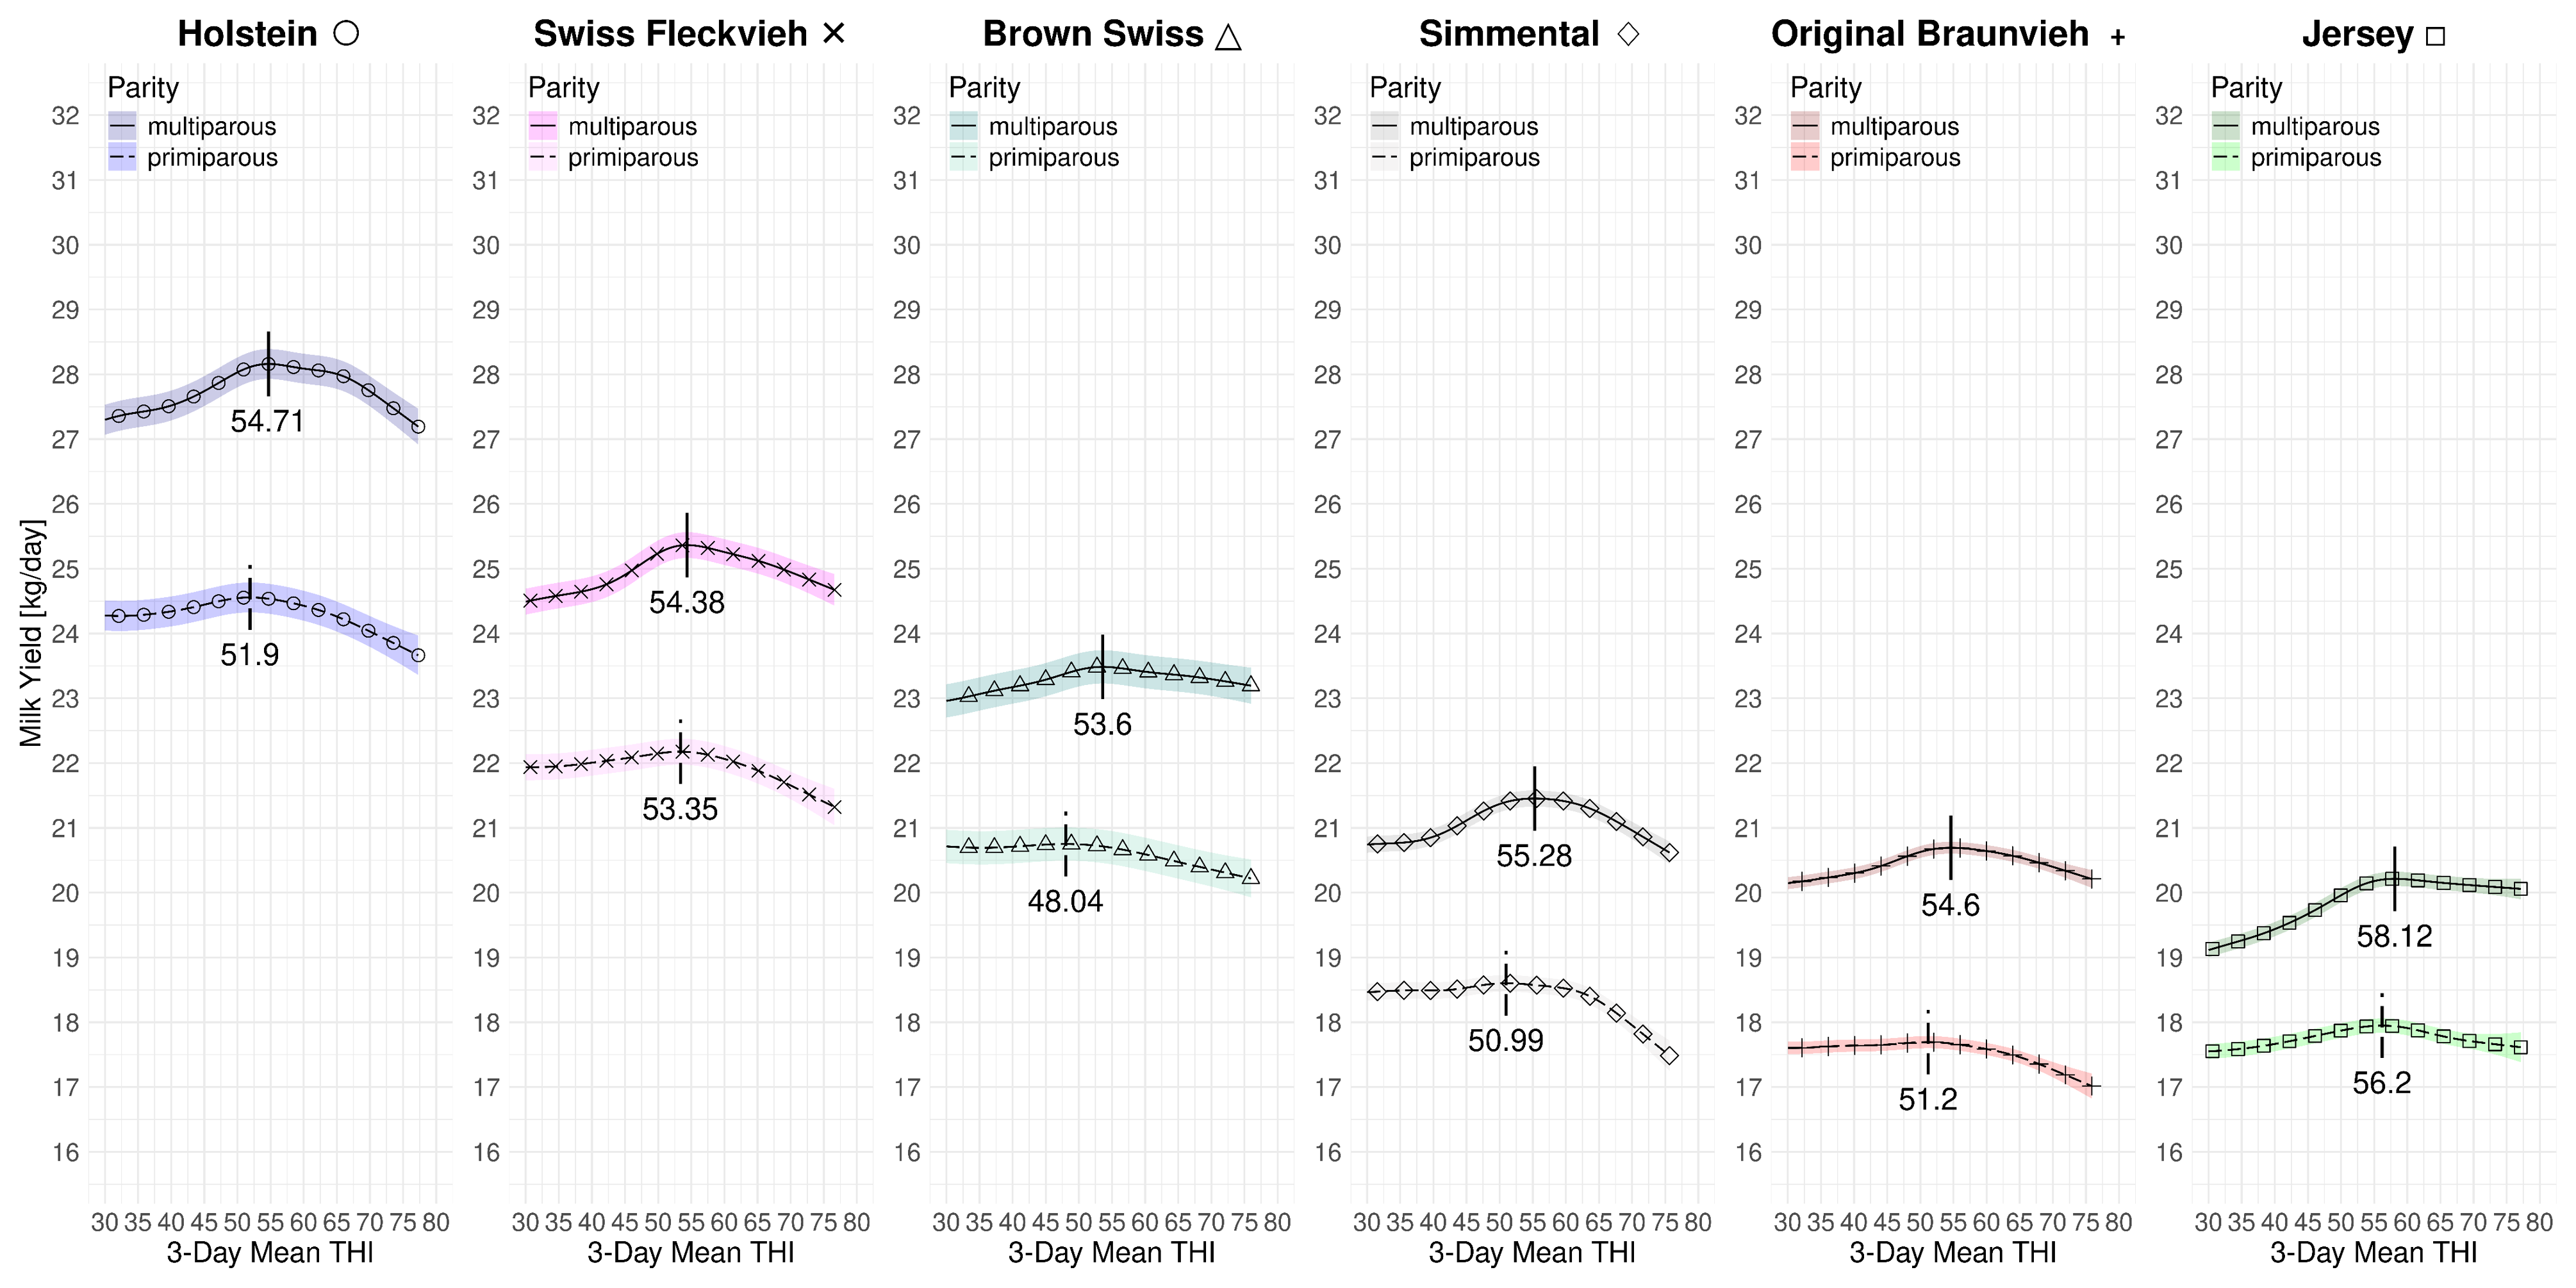
\includegraphics[width=0.85\paperheight]{thesis/figures/results/milk_yield.png}
    
    \caption{3-day mean THI effect on milk yield for primi- and multiparous Swiss dairy cows at 2023 levels with data subsamples covering the full time period from 1983-2023.}
    \label{fig:results_milk_yield}
\end{figure}
\begin{textblock*}{2cm}(20cm, \dimexpr\paperheight/2)
  \rotatebox{90}{\thepage}
\end{textblock*}
\end{landscape}
\newpage
Figure~\ref{fig:results_milk_yield} summarizes the effect of the 3-day mean THI on the volumetric milk yield for both parities and all breeds at average 2023 levels. The subplots are in descending order with respect to the average yields with the high-yield Holstein yield on the left and the modest-yield Jersey breed on the right. Table~\ref{table:milk_yield_full_period} provides a summary of the THI turning points and the associated loss rates. For multiparous cows the peak THI points range from 53.6 for Brown Swiss to 58.12 for Jersey. The THI difference between the lowest and highest peak point is 4.56 THI points. For primiparous cows the the lowest THI peak point is 48.04 for Brown Swiss and 56.2 for Jersey. The THI difference between the lowest and highest peak point for primiparous cows is 8.16 points. In both cases, for Brown Swiss and Jersey, the curves for primi- and multiparous cows, the marginal losses are less accentuated than for the other breeds. For primiparous Simmental we observe a steep drop after a relatively stable period beyond the THI turning point. Figure~\ref{fig:results_milk_marginal_parimiprous} and Figure~\ref{fig:results_milk_marginal_multiparous} only depict the marginal effects of THI without adding the average levels of year and parity. We observe a two-stage decrease for multiparous Holsteins: similarly as for primiparous Simmental, the milk yield decline starts at a THI of 54.71 at a moderate rate. Then, at an approximate value of 65, the loss rate is more steep.

\begin{table}[htbp]
    \centering
    % Define 12 columns
    \begin{tabular}{c c c c c c c c c c c c}
        \toprule
        % First header row
        \multirow{2}{*}{Details} &
        \multirow{2}{*}{\textbf{Breed}} &
        \multirow{2}{*}{\textbf{Period}} &
        \multicolumn{2}{c}{\textbf{THI Peak}} &
        \multicolumn{2}{c}{\textbf{DIM Peak}} &
        \multicolumn{2}{c}{\textbf{THI Loss Rate}} &
        \multicolumn{2}{c}{$\mathbf{R^2}$} \\
        \cmidrule(lr){4-5} \cmidrule(lr){6-7} \cmidrule(lr){8-9} \cmidrule(lr){10-11}
        % Second header row
        & & &
        \textbf{P} & \textbf{M} &
        \textbf{P} & \textbf{M} &
        \textbf{P} & \textbf{M} &
        $\mathbf{R^2_m}$ & $\mathbf{R^2_c}$ & \\
        \hline
        \hline
        % Data rows (replace with your actual data)
        \textcolor{blue}{\ref{model:ho_milk_full}}& HO & Full & 51.90 & 54.71 & 37 & 31 & -0.035 & -0.043 & 0.12 & 0.95\\
        \textcolor{blue}{\ref{model:sf_milk_full}}& SF & Full & 53.35 & 54.38 & 30 & 25 & -0.037 & -0.031 & 0.07 & 0.93\\
        \textcolor{blue}{\ref{model:bs_milk_full}}& BS & Full & 48.04 & 53.60 & 21 & 20 & -0.019 & -0.013 & 0.10 & 0.95\\
        \textcolor{blue}{\ref{model:si_milk_full}}& SI & Full & 50.99 & 55.28 & 26 & 21 & -0.045 & -0.041 & 0.04 & 0.94\\
        \textcolor{blue}{\ref{model:ob_milk_full}}& OB & Full & 51.20 & 54.60 & 24 & 20 & -0.027 & -0.023 & 0.07 & 0.96\\
        \textcolor{blue}{\ref{model:je_milk_full}}& JE & Full & 56.20 & 58.12 & 31 & 25 & -0.016 & -0.008 & 0.14 & 0.95\\
        % Add more data rows as needed
        \bottomrule
    \end{tabular}
    \caption{Milk Yield - Full Period - Turning Points and Loss Rates}
    \label{table:milk_yield_full_period}
\end{table}

\begin{figure}[H]
    \centering
    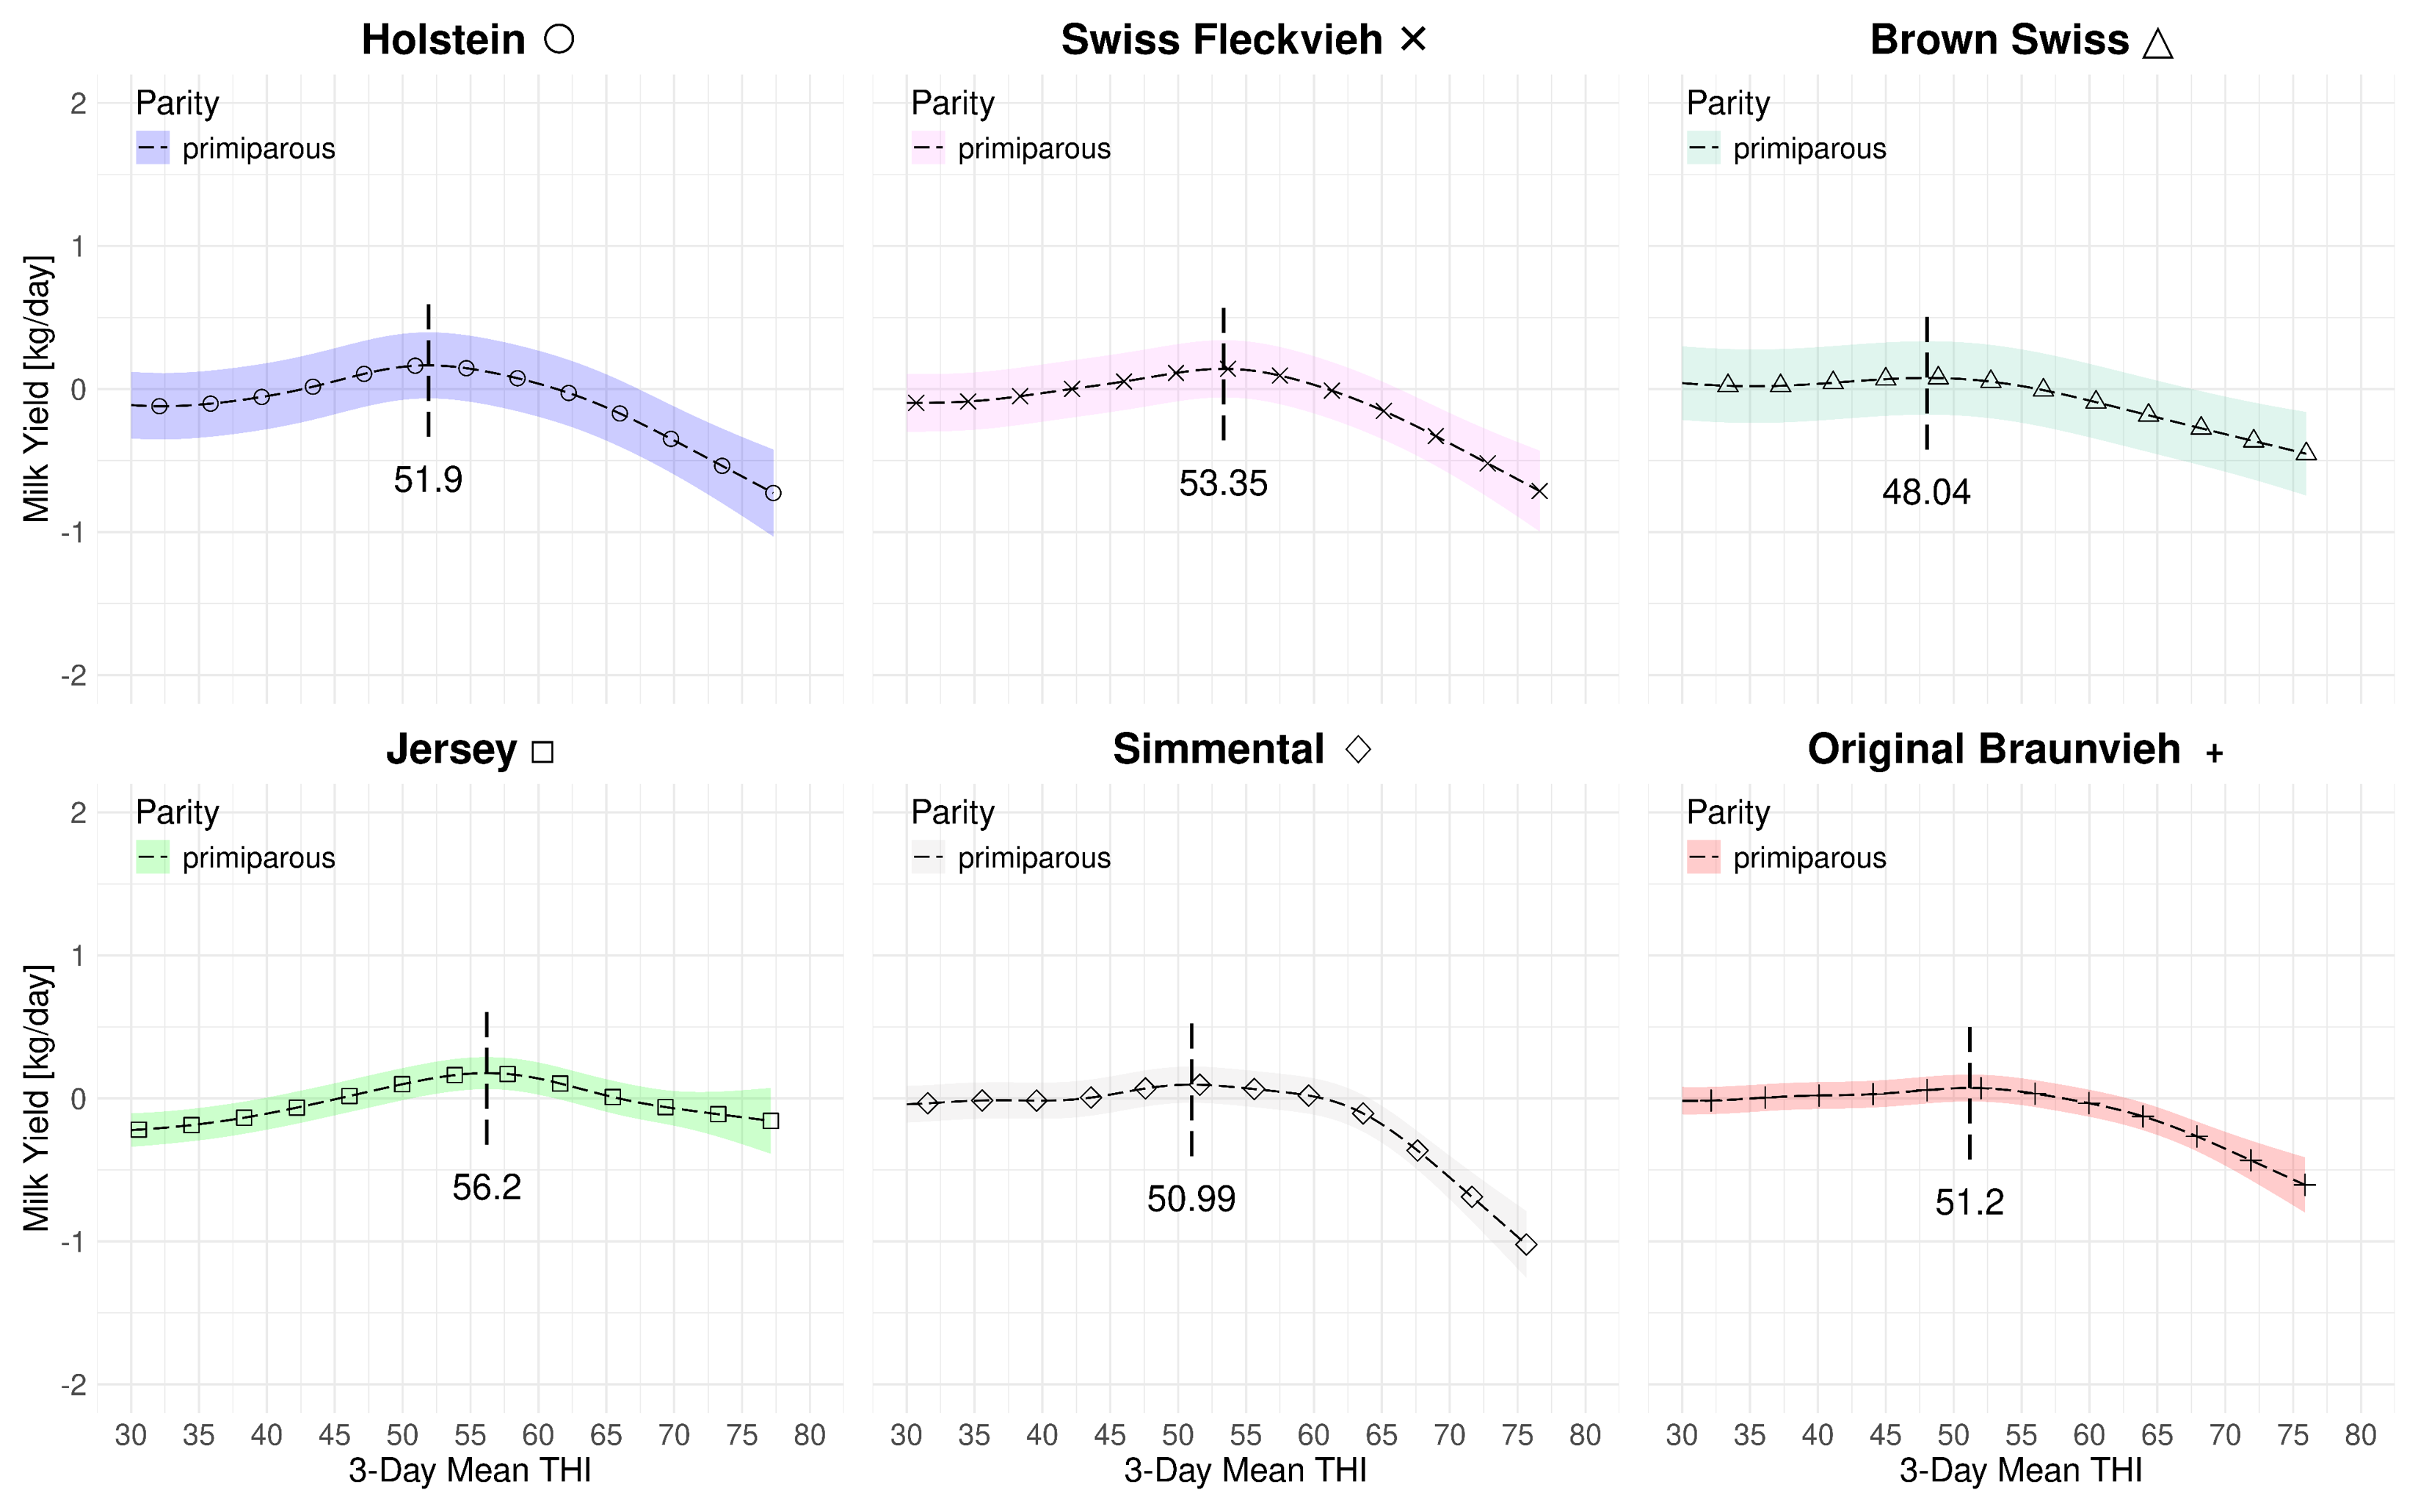
\includegraphics[width=\textwidth]{thesis/figures/results/milk_yield_marginal_primi.png}
    \caption{3-day mean marginal THI effect on milk yield for primiparous Swiss dairy cows at 2023 levels with data subsamples covering the full time period from 1982-2023.}
    \label{fig:results_milk_marginal_parimiprous}
\end{figure}

\begin{figure}[H]
    \centering
    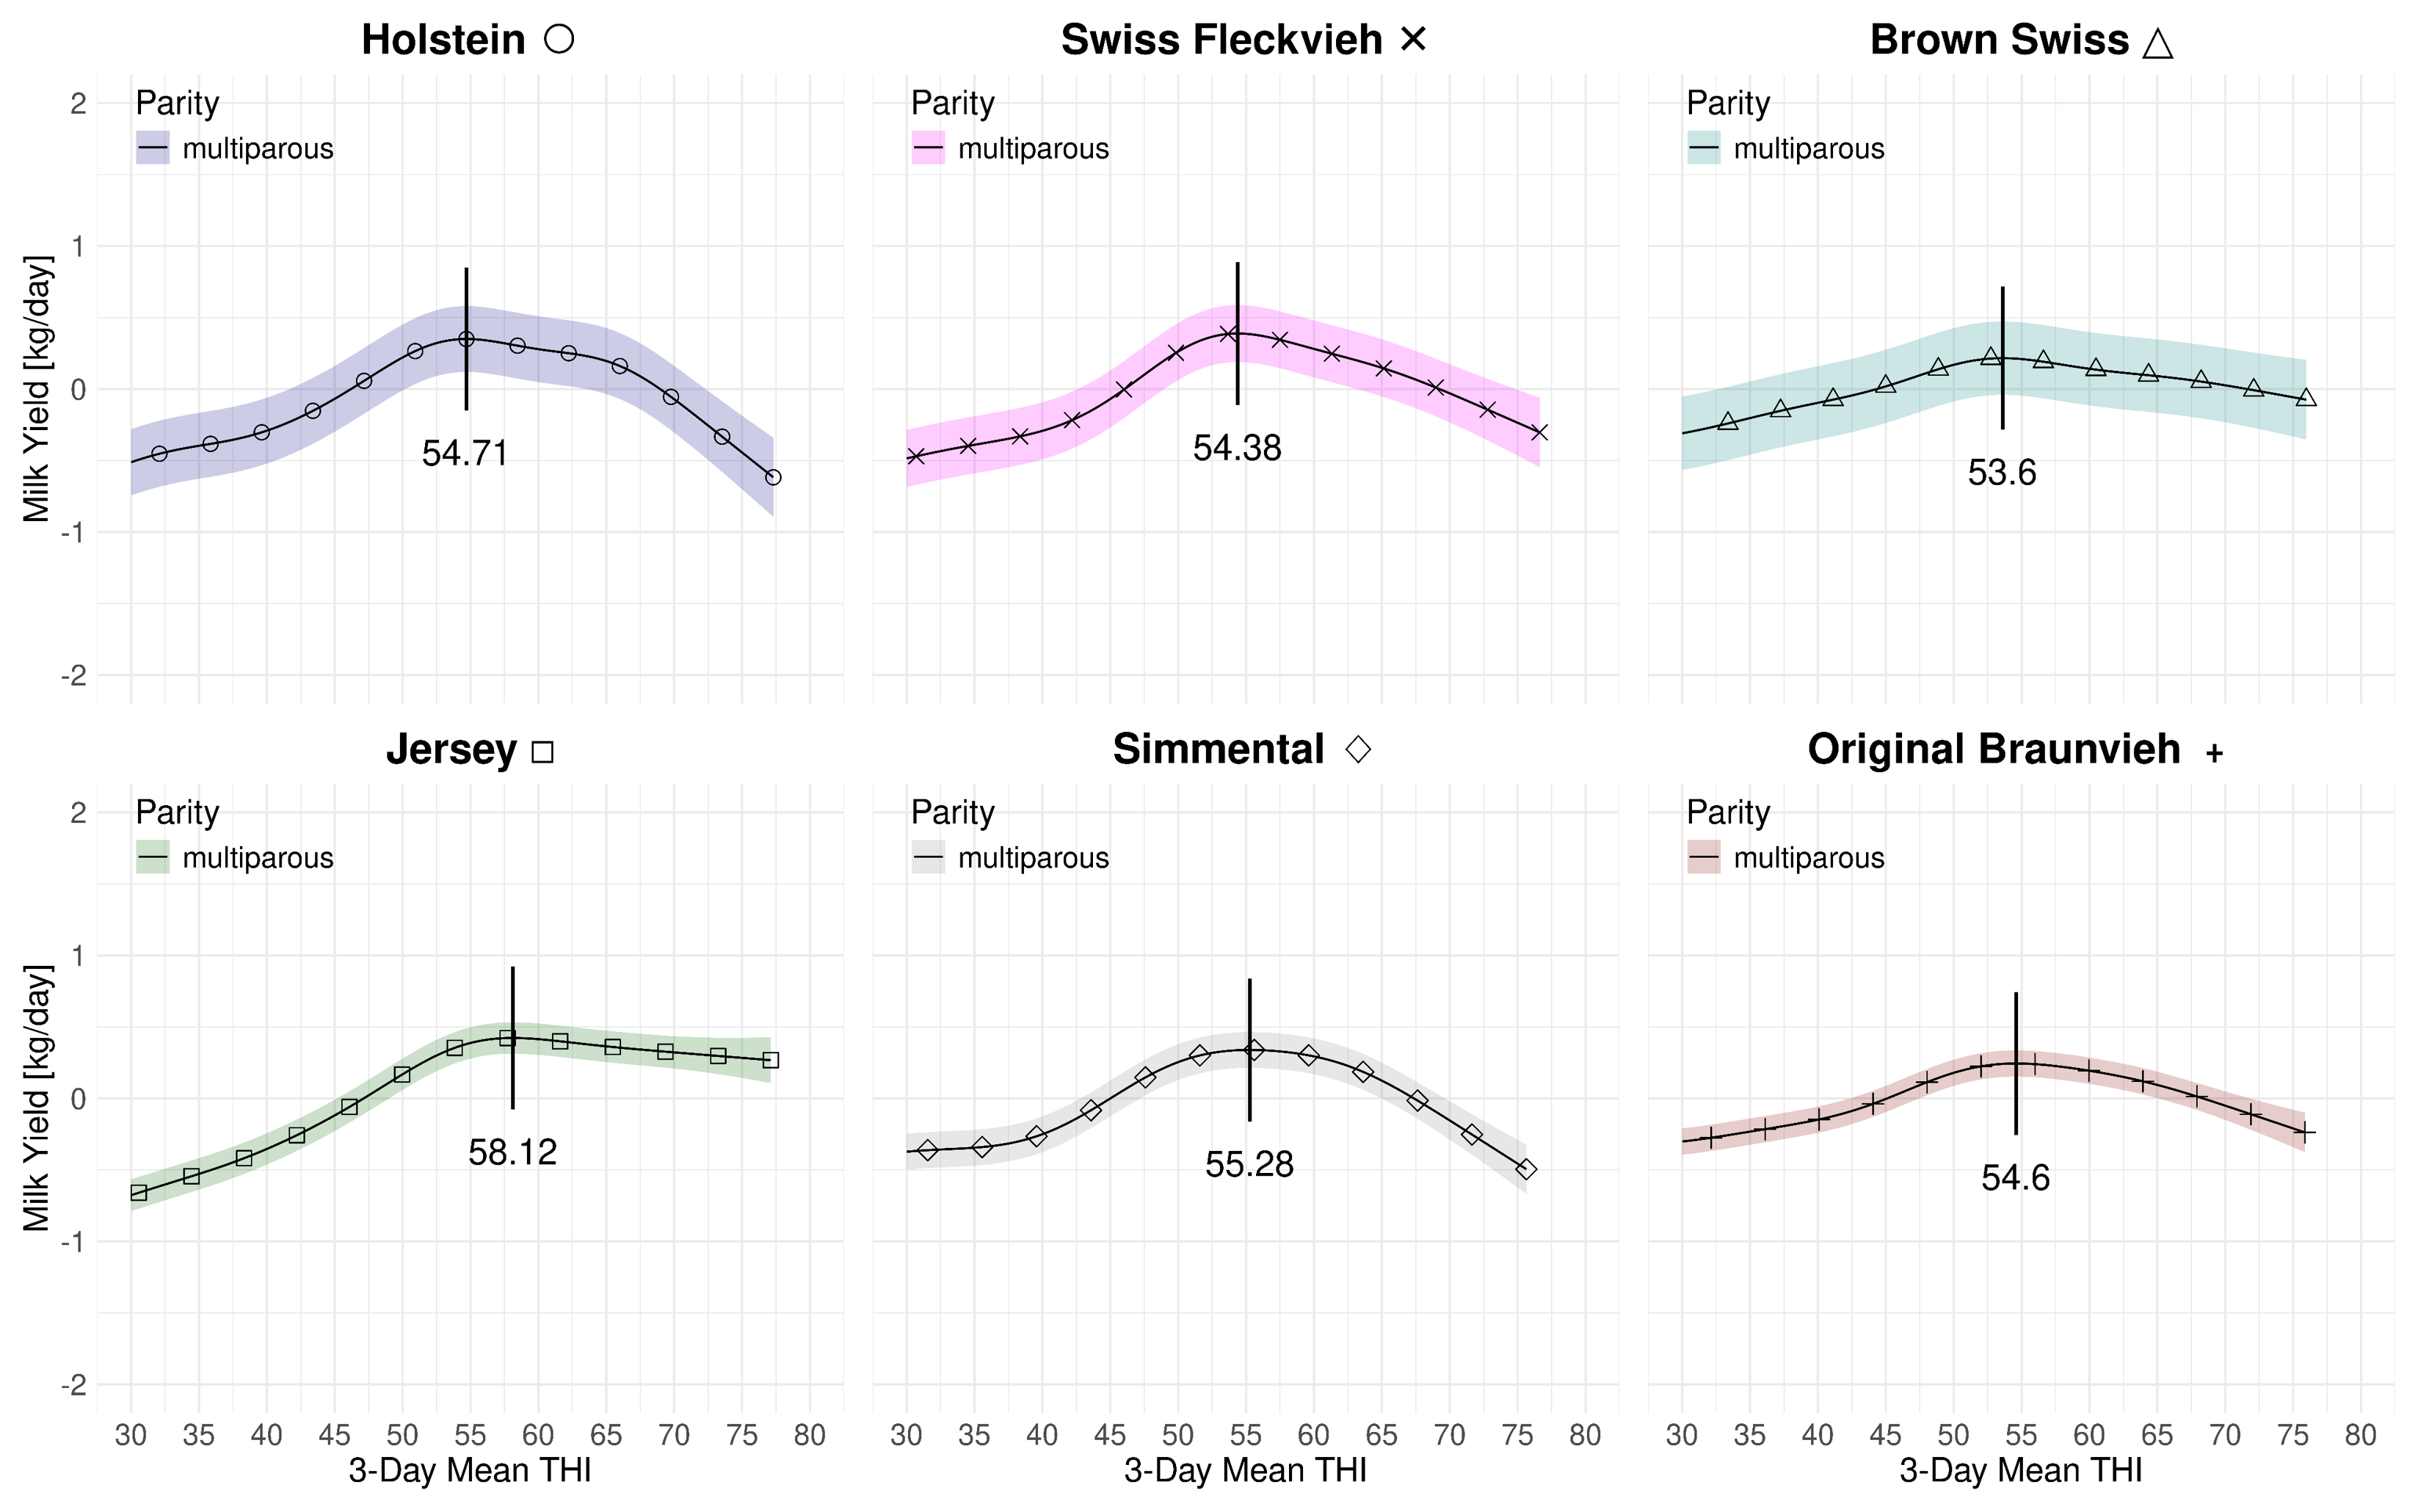
\includegraphics[width=\textwidth]{thesis/figures/results/milk_yield_marginal_multi.png}
    
    \caption{3-day mean marginal THI effect on milk yield for multiparous Swiss dairy cows at 2023 levels with data subsamples covering the full time period from 1982-2023.}
    \label{fig:results_milk_marginal_multiparous}
\end{figure}


    
\newpage

\newpage
\begin{landscape}
    \thispagestyle{empty}
    \section{ECM Yield}\label{sec:ecm_yield}
    \begin{figure}[ht]
        \centering
        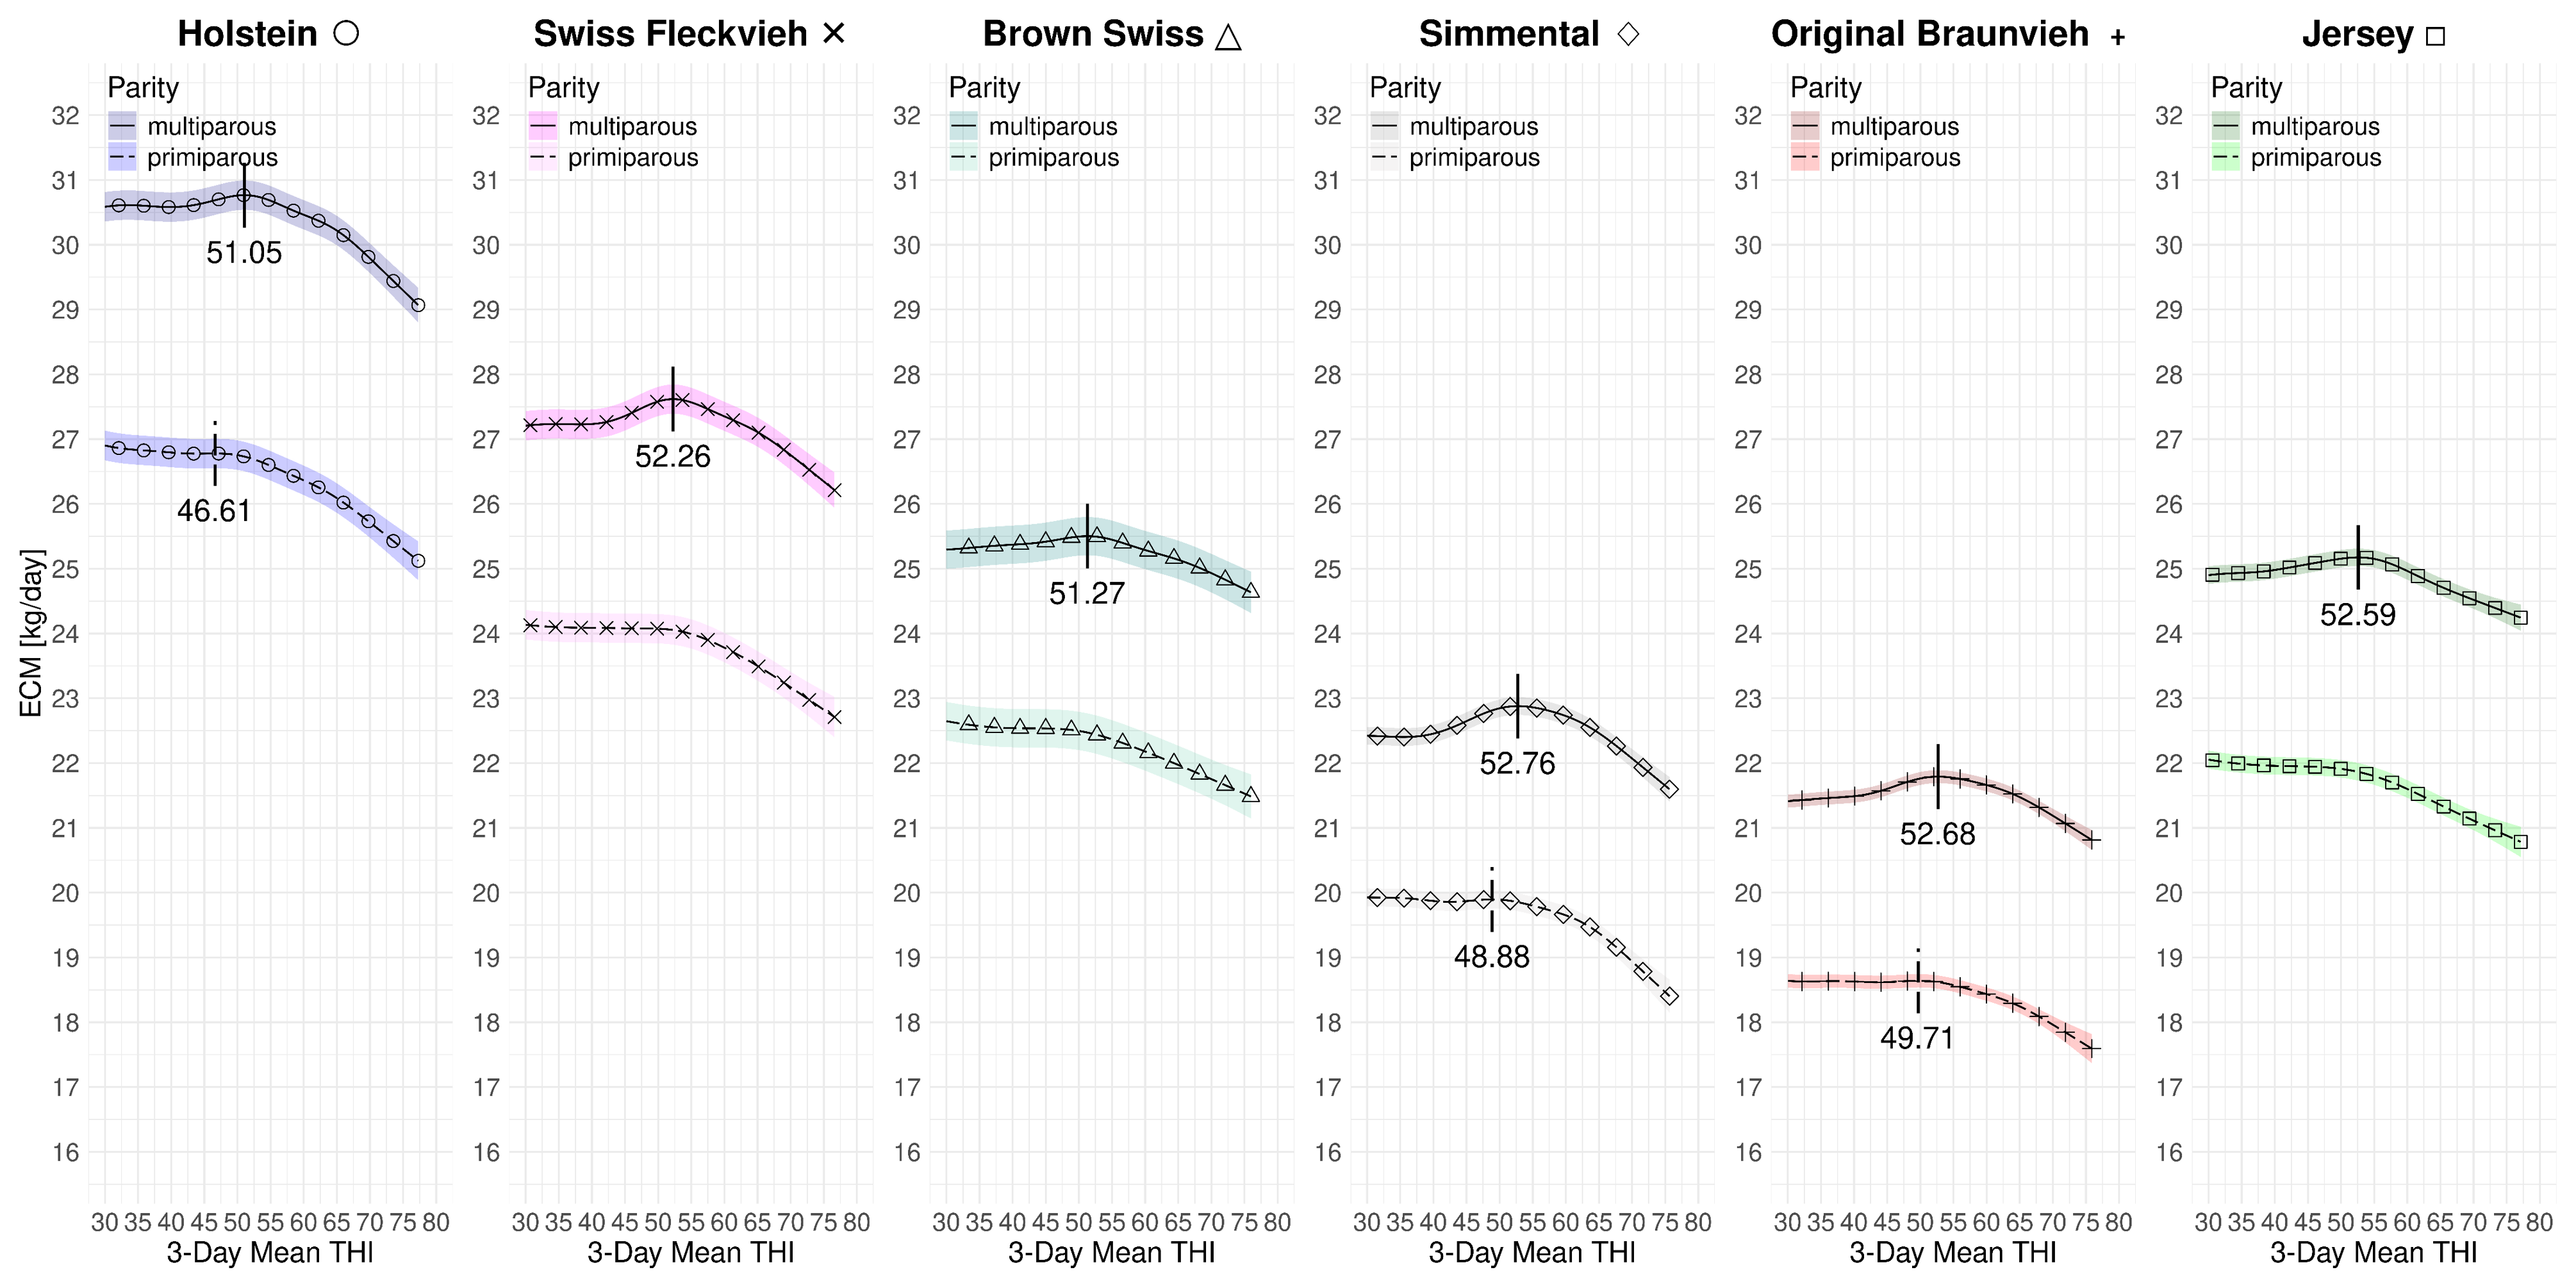
\includegraphics[width=0.85\paperheight]{thesis/figures/results/ecm_yield.png}
        \caption{3-day mean THI effect on ECM yield for primi- and multiparous Swiss dairy cows at 2023 levels with data subsamples covering the full time period from 1983-2023.}
        \label{fig:results_ecm_yield}
    \end{figure}
    
    \begin{textblock*}{2cm}(20cm, \dimexpr\paperheight/2)
    \rotatebox{90}{\thepage}
    \end{textblock*}
\end{landscape}
\newpage


Figure~\ref{fig:results_ecm_yield} summarizes the effect of the 3-day mean THI on the component-corrected milk yield for both parities and all breeds at average 2023 levels. Hence, the milk yield is normalized with respect to fat and protein. First, by the definition of ECM, the average yield levels increase for all breeds\footnote{The average milk and ECM yield levels of 2023 derived with descriptive statistics can be consulted in Table~\ref{table:average_breed_performance_2023}}. The jump for Jersey cows is expected since they are known as a high-fat and high-protein breed. Moreover, we are able to identify turning points for all breeds in the multiparous case. The lowest THI peak is at 51.05 for Holstein and the highest at 52.76 for Simmental. The difference between the lowest and highest THI peak point is 1.71. For primiparous cows, we cannot identify the THI turning points for Swiss Fleckvieh, Brown Swiss and Jersey. This is because their corresponding slopes are continuously decreasing. Therefore, from a numerical perspective, there are no turning points in these cases. However, in all three cases, fairly steep changes in the loss rates at THI values in the mid-fifties are identifiable. For the other three breeds with available turning points, these are Holstein (46.61), Simmental (48.88) and Original Braunvieh (49.71). Among them, the difference between the lowest and highest turning point is 3.41 THI points. Table~\ref{table:ecm_yield_full_period} lists the individual THI turning points. Figure~\ref{fig:results_ecm_marginal_parimiprous} and Figure~\ref{fig:results_ecm_marginal_multiparous} solely visualize the marginal effects of THI on ECM yield in separate subfigures for primi- and multiparous cows.

\begin{table}[htbp]
    \centering
    % Define 12 columns
    \begin{tabular}{c c c c c c c c c c c c}
        \toprule
        % First header row
        \multirow{2}{*}{Details} &
        \multirow{2}{*}{\textbf{Breed}} &
        \multirow{2}{*}{\textbf{Period}} &
        \multicolumn{2}{c}{\textbf{THI Peak}} &
        \multicolumn{2}{c}{\textbf{DIM Peak}} &
        \multicolumn{2}{c}{\textbf{THI Loss Rate}} &
        \multicolumn{2}{c}{$\mathbf{R^2}$} \\
        \cmidrule(lr){4-5} \cmidrule(lr){6-7} \cmidrule(lr){8-9} \cmidrule(lr){10-11}
        % Second header row
        & & &
        \textbf{P} & \textbf{M} &
        \textbf{P} & \textbf{M} &
        \textbf{P} & \textbf{M} &
        $\mathbf{R^2_m}$ & $\mathbf{R^2_c}$ & \\
        \hline
        \hline
        % Data rows (replace with your actual data)
        \textcolor{blue}{\ref{model:ho_ecm_full}}& HO & Full & 46.61 & 51.05 & 13 & 20 & -0.054 & -0.065 & 0.06 & 0.89\\
        \textcolor{blue}{\ref{model:sf_ecm_full}}& SF & Full & - & 52.26 & 11 & - & - & -0.058 & 0.07 & 0.90\\
        \textcolor{blue}{\ref{model:bs_ecm_full}}& BS & Full & - & 51.27 & 13 & 8 & - & -0.035 & 0.06 & 0.92\\
        \textcolor{blue}{\ref{model:si_ecm_full}}& SI & Full & 48.88 & 52.76 & 9 & - & -0.056 & -0.056 & 0.03 & 0.93\\
        \textcolor{blue}{\ref{model:ob_ecm_full}}& OB & Full & 49.71 & 52.68 & 14 & 4 & -0.042 & -0.040 & 0.04 & 0.92\\
        \textcolor{blue}{\ref{model:je_ecm_full}}& JE & Full & - & 52.59 & 22 & 23 & - & -0.038 & 0.07 & 0.90\\
        % Add more data rows as needed
        \bottomrule
    \end{tabular}
    \caption{ECM Yield - Full Period - Turning Points and Loss Rates}
    \label{table:ecm_yield_full_period}
\end{table}

\begin{figure}[H]
    \centering
    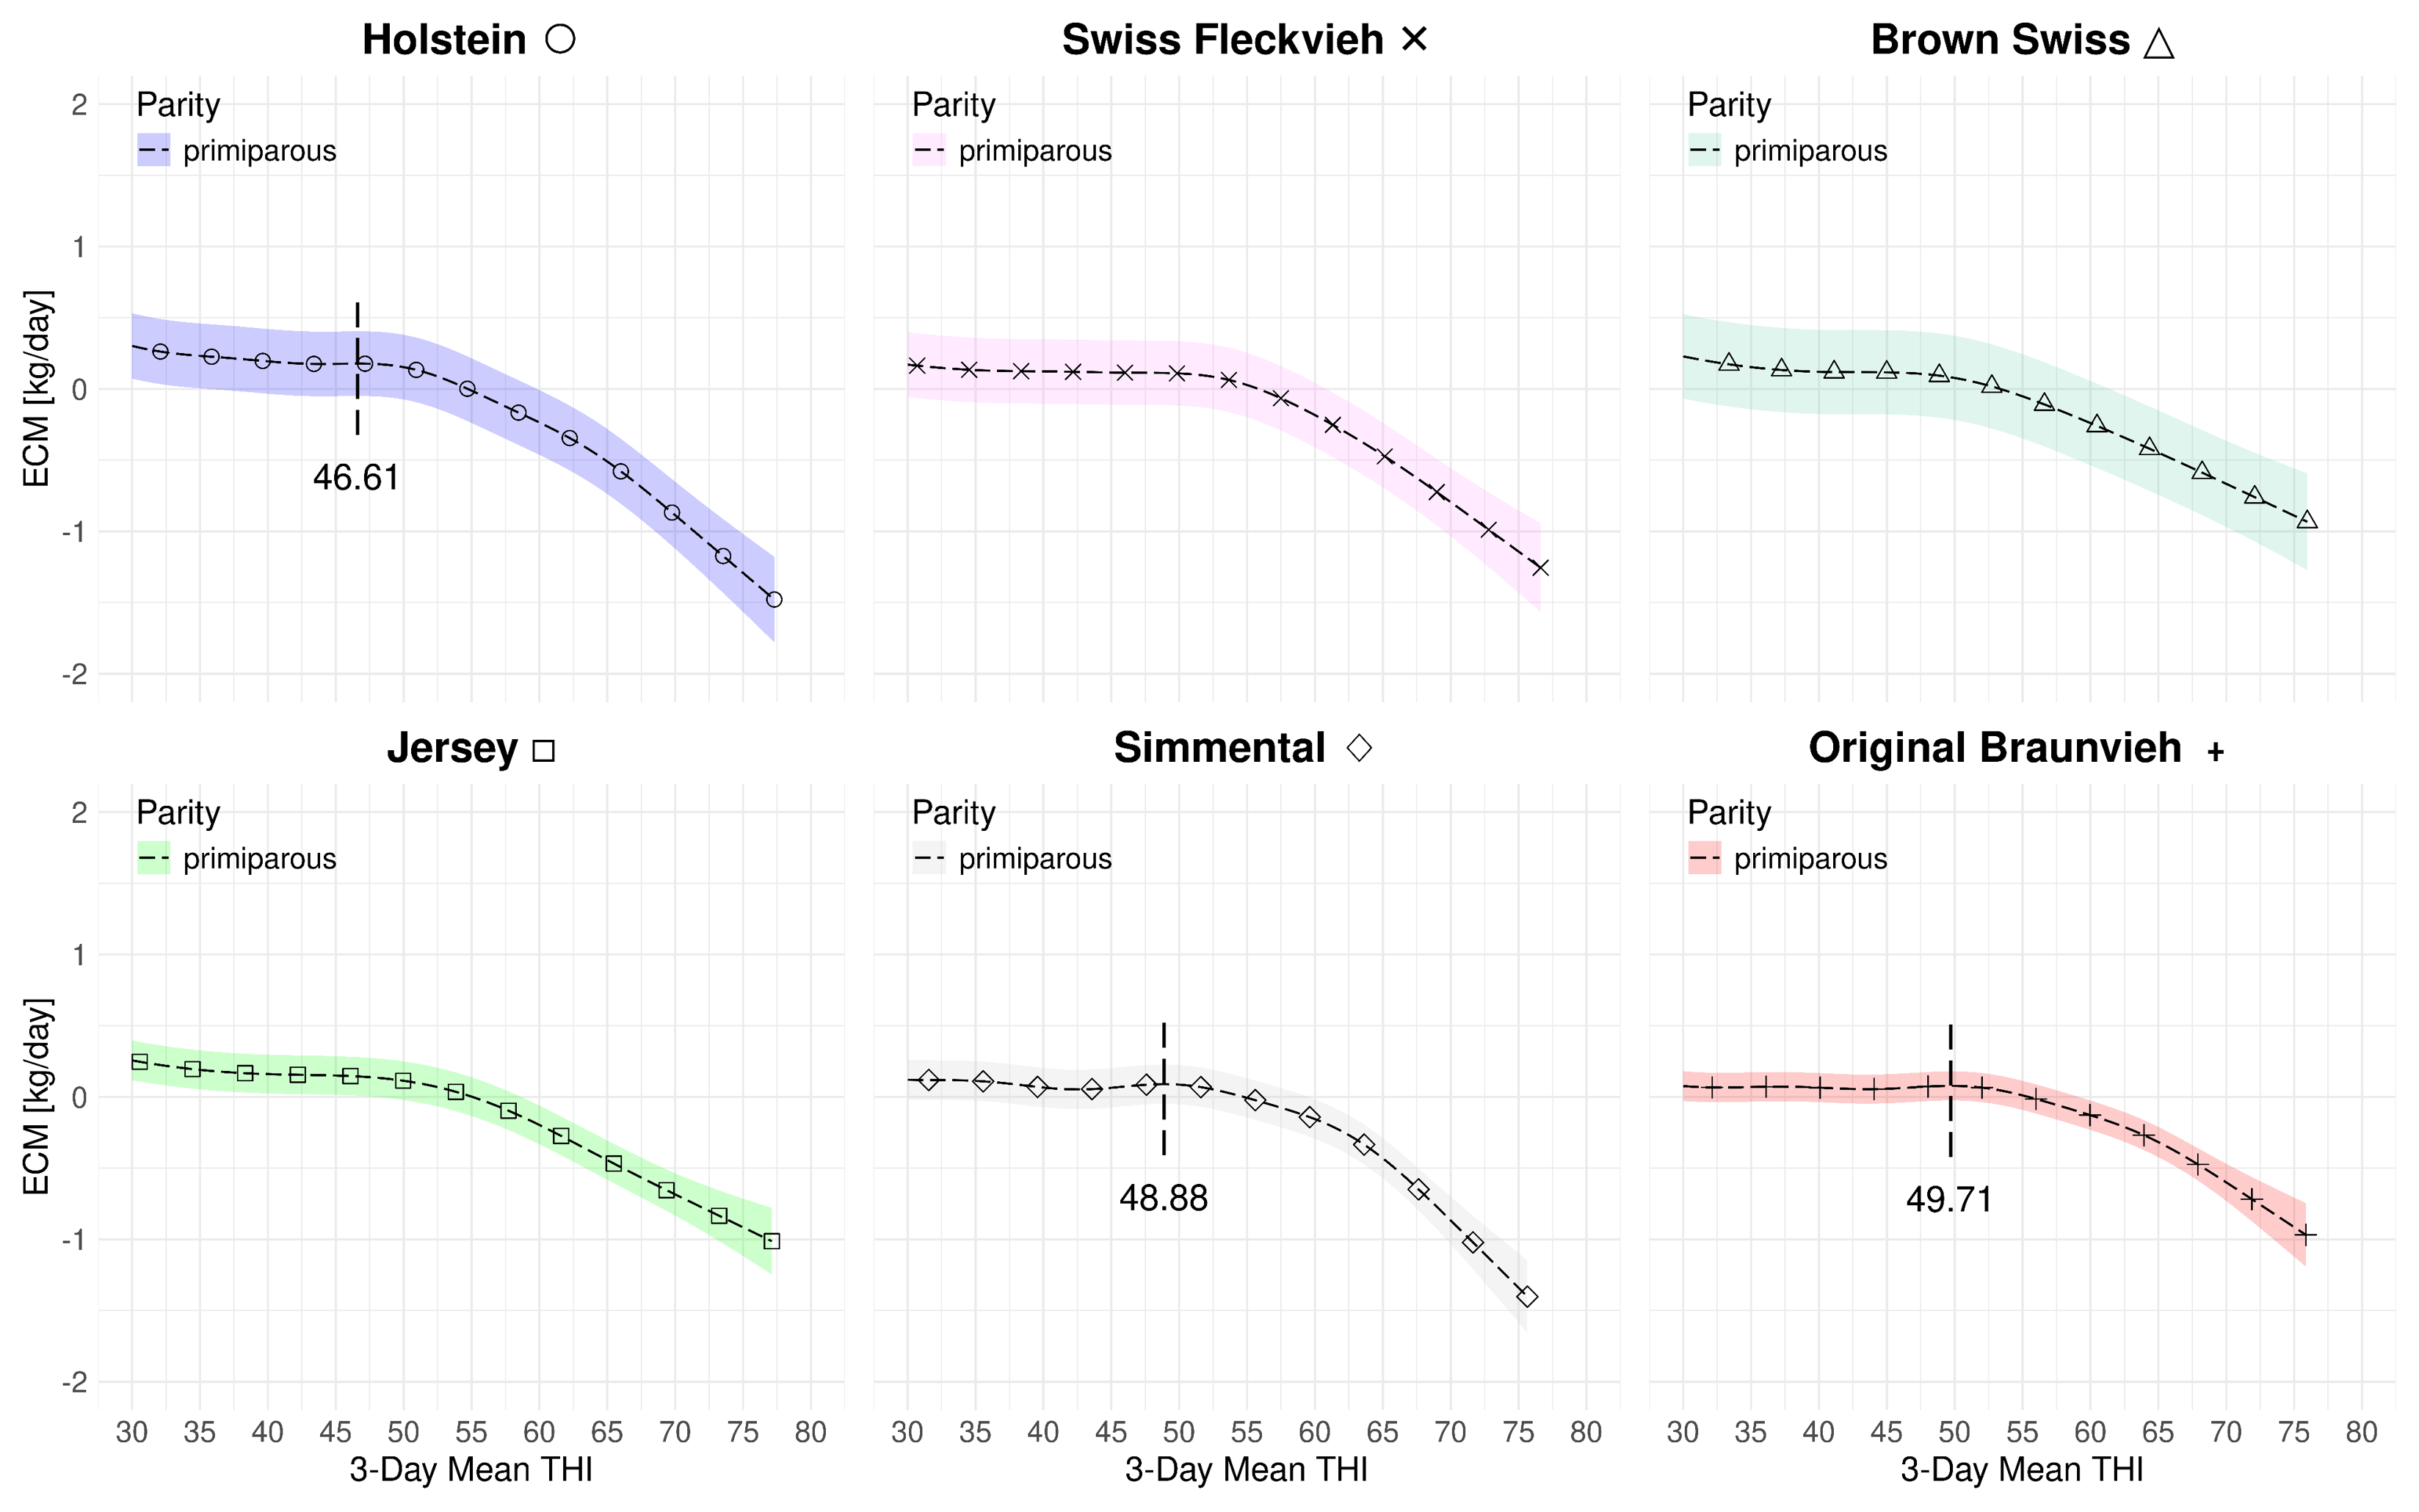
\includegraphics[width=\textwidth]{thesis/figures/results/ecm_yield_marginal_primi.png}
    \caption{3-day mean marginal THI effect on ECM yield for primiparous Swiss dairy cows at 2023 levels with data subsamples covering the full time period from 1983-2023.}
    \label{fig:results_ecm_marginal_parimiprous}
\end{figure}

\begin{figure}[H]
    \centering
    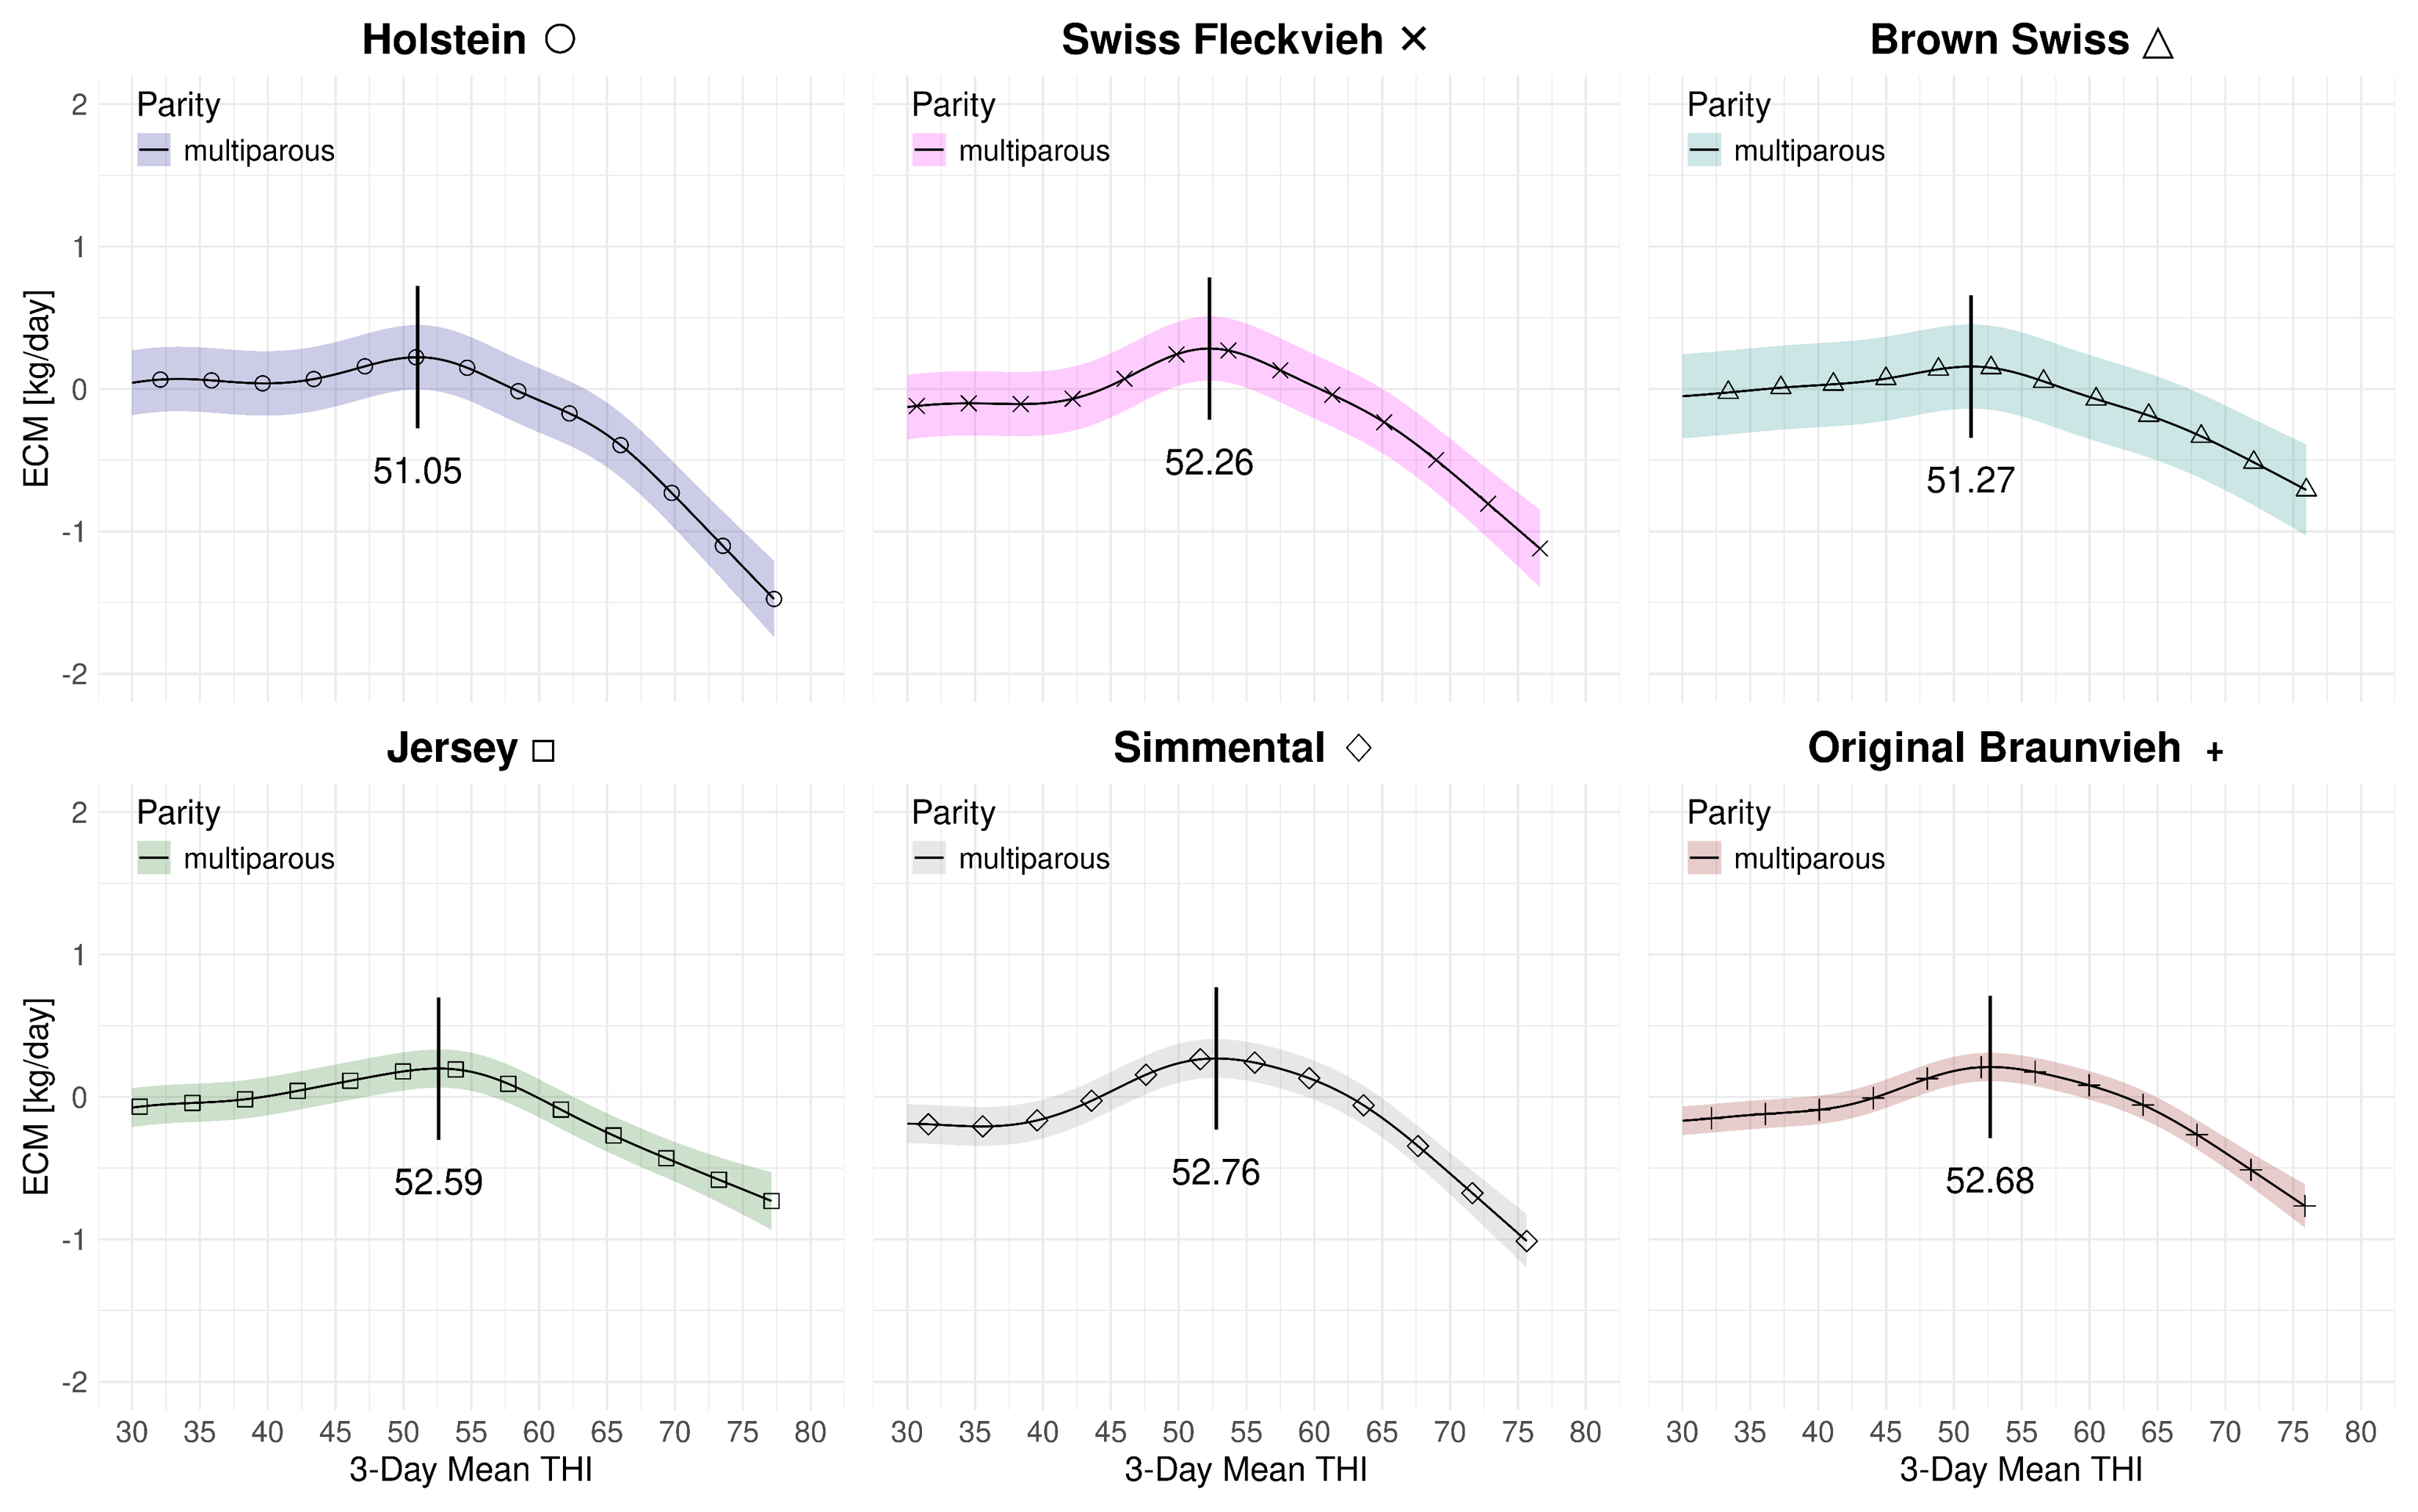
\includegraphics[width=\textwidth]{thesis/figures/results/ecm_yield_marginal_multi.png}
    
    \caption{3-day mean marginal THI effect on ECM yield for multiparous Swiss dairy cows at 2023 levels with data subsamples covering the full time period from 1983-2023.}
    \label{fig:results_ecm_marginal_multiparous}
\end{figure}



\newpage

\section{Split Period: Until 2010 - After 2010}\label{sec:split_period}
Table~\ref{table:milk_yield_split_period} and Table~\ref{table:ecm_yield_split_period} compare the THI turning points and loss rates for the split-period experiments. The associated figures are provided in Appendix~\ref{appendix:split_period}. We observe THI turning point shifts between the two periods. More specifically, the turning points are at lower THI values in the period 2011-2023. However, in many cases, leftward turning point shifts, come with lower linearized loss rates.

% Second Table
\begin{table}[htbp]
    \centering
    % Define 12 columns
    \begin{tabular}{c c c c c c c c c c c c}
        \toprule
        % First header row
        \multirow{2}{*}{Details} &
        \multirow{2}{*}{\textbf{Breed}} &
        \multirow{2}{*}{\textbf{Period}} &
        \multicolumn{2}{c}{\textbf{THI Peak}} &
        \multicolumn{2}{c}{\textbf{DIM Peak}} &
        \multicolumn{2}{c}{\textbf{THI Loss Rate}} &
        \multicolumn{2}{c}{$\mathbf{R^2}$} \\
        \cmidrule(lr){4-5} \cmidrule(lr){6-7} \cmidrule(lr){8-9} \cmidrule(lr){10-11}
        % Second header row
        & & &
        \textbf{P} & \textbf{M} &
        \textbf{P} & \textbf{M} &
        \textbf{P} & \textbf{M} &
        $\mathbf{R^2_m}$ & $\mathbf{R^2_c}$ & \\
        \hline
        \hline
        % Data rows (replace with your actual data)
        \textcolor{blue}{\ref{model:ho_milk_before}}& HO & $\leq 2010$ & 53.40 & 55.24 & 35 & 28 & -0.040 & -0.041 & 0.06 & 0.94\\
        \textcolor{blue}{\ref{model:ho_milk_after}}& HO & $>2010$ & 51.19 & 54.83 & 37 & 33 & -0.031 & -0.040 & 0.12 & 0.95\\
        \hline
        \textcolor{blue}{\ref{model:sf_milk_before}}& SF & $\leq 2010$ & 54.00 & 54.34 & 29 & 24 & -0.033 & -0.033 & 0.05 & 0.93\\
        \textcolor{blue}{\ref{model:sf_milk_after}}& SF & $>2010$ & 51.75 & 54.62 & 35 & 28 & -0.023 & -0.010 & 0.07 & 0.94\\
        \hline
        \textcolor{blue}{\ref{model:bs_milk_before}}& BS & $\leq 2010$ & 52.40 & 53.67 & 21 & 20 & -0.024 & -0.028 & 0.08 & 0.95\\
        \textcolor{blue}{\ref{model:bs_milk_after}}& BS & $>2010$ & 46.76 & 51.83 & 26 & 22 & -0.021 & -0.006 & 0.10 & 0.95\\
        \hline
        \textcolor{blue}{\ref{model:si_milk_before}}& SI & $\leq 2010$ & 52.26 & 55.80 & 25 & 20 & -0.034 & -0.026 & 0.03 & 0.93\\
        \textcolor{blue}{\ref{model:si_milk_after}}& SI & $>2010$ & 53.10 & 55.35 & 28 & 22 & -0.023 & -0.013 & 0.03 & 0.94\\
        \hline
        \textcolor{blue}{\ref{model:ob_milk_before}}& OB & $\leq 2010$ & 52.73 & 55.01 & 23 & 20 & -0.028 & -0.025 & 0.04 & 0.95\\
        \textcolor{blue}{\ref{model:ob_milk_after}}& OB & $>2010$ & 49.49 & 52.63 & 29 & 21 & -0.023 & -0.019 & 0.06 & 0.94\\
        \hline
        \textcolor{blue}{\ref{model:je_milk_before}}& JE & $\leq 2010$ & 57.09 & 58.33 & 27 & 22 & -0.019 & -0.021 & 0.10 & 0.96\\
        \textcolor{blue}{\ref{model:je_milk_after}}& JE & $>2010$ & 55.06 & 58.13 & 33 & 27 & -0.015 & -0.007 & 0.12 & 0.95\\            
        % Add more data rows as needed
        \bottomrule
    \end{tabular}
    \caption{Milk Yield - Split Period - Turning Points and Loss Rates}
    \label{table:milk_yield_split_period}
\end{table}

% Second Table
\begin{table}[htbp]
    \centering
    % Define 12 columns
    \begin{tabular}{c c c c c c c c c c c c}
        \toprule
        % First header row
        \multirow{2}{*}{Details} &
        \multirow{2}{*}{\textbf{Breed}} &
        \multirow{2}{*}{\textbf{Period}} &
        \multicolumn{2}{c}{\textbf{THI Peak}} &
        \multicolumn{2}{c}{\textbf{DIM Peak}} &
        \multicolumn{2}{c}{\textbf{THI Loss Rate}} &
        \multicolumn{2}{c}{$\mathbf{R^2}$} \\
        \cmidrule(lr){4-5} \cmidrule(lr){6-7} \cmidrule(lr){8-9} \cmidrule(lr){10-11}
        % Second header row
        & & &
        \textbf{P} & \textbf{M} &
        \textbf{P} & \textbf{M} &
        \textbf{P} & \textbf{M} &
        $\mathbf{R^2_m}$ & $\mathbf{R^2_c}$ & \\
        \hline
        \hline
        % Data rows (replace with your actual data)
        
        \textcolor{blue}{\ref{model:ho_ecm_before}}& HO & $\leq 2010$ & 48.48 & 51.40 & 15 & - & -0.057 & -0.060 & 0.07 & 0.88\\
        \textcolor{blue}{\ref{model:ho_ecm_after}}& HO & $>2010$ & 47.49 & 50.05 & 23 & 15 & -0.054 & -0.059 & 0.06 & 0.89\\
        \hline
        \textcolor{blue}{\ref{model:sf_ecm_before}}& SF & $\leq 2010$ & 50.05 & 52.27 & - & - & -0.047 & -0.059 & 0.06 & 0.90\\
        \textcolor{blue}{\ref{model:sf_ecm_after}}& SF & $>2010$ & 47.96 & 50.30 & 19 & 10 & -0.045 & -0.035 & 0.04 & 0.88\\
        \hline
        \textcolor{blue}{\ref{model:bs_ecm_before}}& BS & $\leq 2010$ & 49.25 & 51.76 & 12 & - & -0.039 & -0.047 & 0.06 & 0.90\\
        \textcolor{blue}{\ref{model:bs_ecm_after}}& BS & $>2010$ & - & 48.03 & 16 & 11 & - & -0.027 & 0.02 & 0.93\\
        \hline
        \textcolor{blue}{\ref{model:si_ecm_before}}& SI & $\leq 2010$ & - & 53.28 & 8 & - & - & -0.044 & 0.05 & 0.90\\
        \textcolor{blue}{\ref{model:si_ecm_after}}& SI & $>2010$ & 48.97 & 52.81 & 12 & - & -0.033 & -0.027 & 0.05 & 0.87\\
        \hline
        \textcolor{blue}{\ref{model:ob_ecm_before}}& OB & $\leq 2010$ & 51.27 & 52.96 & 12 & - & -0.034 & -0.040 & 0.03 & 0.92\\
        \textcolor{blue}{\ref{model:ob_ecm_after}}& OB & $>2010$ & - & 51.07 & 16 & 9 & - & -0.033 & 0.03 & 0.89\\
        \hline
        \textcolor{blue}{\ref{model:je_ecm_before}}& JE & $\leq 2010$ & - & 51.73 & 20 & 21 & - & -0.045 & 0.07 & 0.93\\
        \textcolor{blue}{\ref{model:je_ecm_after}}& JE & $>2010$ & 46.57 & 52.72 & 25 & 24 & -0.037 & -0.038 & 0.09 & 0.92\\
        % Add more data rows as needed
        \bottomrule
    \end{tabular}
    \caption{ECM Yield - Split Period - Turning Points and Loss Rates}
    \label{table:ecm_yield_split_period}
\end{table}

\newpage
\begin{landscape}
    \thispagestyle{empty}
    \section{Discussion}\label{sec:discussion}
    \begin{figure}[ht]
        \centering
        \includegraphics[width=0.85\paperheight]{thesis/figures/results/ecm_milk_combined.png}
        \caption{3-day mean THI effect on milk yield and ECM yield for primi- and multiparous Swiss dairy cows at 2023 levels with data subsamples covering the full time period from 1982-2023. This figure combines Figure~\ref{fig:results_milk_yield} and Figure~\ref{fig:results_ecm_yield}.}
        \label{fig:ecm_milk_combined}
    \end{figure}
    
    \begin{textblock*}{2cm}(20cm, \dimexpr\paperheight/2)
    \rotatebox{90}{\thepage}
    \end{textblock*}
\end{landscape}
\newpage

\paragraph{General Observations} Figure~\ref{fig:ecm_milk_combined} combines the findings of the full-period models presented in Section~\ref{sec:milk_yiled} and Section~\ref{sec:ecm_yield}. Consistent with expectations, non-linear effects THI on milk yield and ECM yield have been identified. Specifically, the observed concave-downward responses of THI align with biological assumptions, indicating that the animals reach an optimal performance level at specific THI points, beyond which their productivity diminishes as THI levels further increase. For the majority of breeds, including both primiparous and multiparous cases, these THI turning points can be numerically determined. Additionally, clear differences in average performance levels across breeds are evident, with Holstein cattle exhibiting superior production, whereas dual-purpose breeds such as Simmental and Original Braunvieh exhibit lower performance metrics, contingent upon whether the yield is adjusted for energy content. Furthermore, it is possible to observe distinct THI turning points among different breeds. In general, the impact of THI on milk yield is moderate in relation to the average yields among different breeds. The effects of accumulated THI, commencing from the turning points, range from approximately 0 to 1.5 kg. None of the breeds appears to exhibit significantly superior performance over others due to THI effects. This observation is congruent with the findings of \cite{ahmed_temperature_2022} that suggest diversification of a dairy cow portfolio does not improve resilience to heat. However, further research is required, employing simulations over extended time frames and including productivity parameters such as cost per cow and breed.

\paragraph{Low THI Values} An initial investigation reveals unexpectedly low THI values at the turning points. It is anticipated that the THI turning points would be situated in the high sixties or early seventies for both milk yield and ECM yield \citep{armstrong_heat_1994, de_rensis_seasonal_2015, vroege_effects_2023}, which correspond to light heat stress and temperatures between 22°C and 33°C, depending on the relative humidity, according to Figure~\ref{fig:thi_table}. Contrary to this expectation, the peak THI values start in the low forties concerning ECM yield for primiparous cows and extend to the high sixties with regard to milk yield for multiparous cows. This implies dairy cows reach their peak performance with respect to THI independent of the lactation stage, at positive single-digit degrees Celsius in some cases. First, we did check our data pipeline multiple times for errors and also ran numerous sanity checks regarding the location-weather matching. Second, in Switzerland, the average farm are small-scale family operations. We speculated that this effect is due to the fact that in Switzerland the average farm is a small-scale family operation. When applying the same models to data solely from larger farms with more than 60 cows in 2023, supposedly well-managed, the results indicate an elevation in THI thresholds by approximately 1-2 points. Employing broken-stick fixed-effect models from econometrics, which account for animals and farms as unobserved heterogeneity and are estimated through pooled OLS regression with a search for the statistically optimal breaking point, yields similar THI threshold values. Furthermore, when using the same methodological framework but substituting mean THI values with maximum THI values, the threshold increases by several THI points; however, all remain significantly below the expected threshold of 68 THI points\footnote{This serves purely as an indicator because pooled OLS is not appropriate for our unbalanced dataset. The notebooks of these fixed effect models are provided in Appendix~\ref{appendix:source_code}. The results must be considered as strongly biased.}. These THI turning points have precedents: \cite{hill_dairy_2015} report average THI values as low as 54.9 as threshold values for outdoor cows. Furthermore, \cite{vinet_estimation_2023} identify optimal 3-day THI ranges between 50 and 55 for the Montbélliarde breed. Finally, our reference study \cite{ahmed_temperature_2022} documents negative marginal effects on milk yield at temperatures of 4-5$^\circ$C based on a 7-day mean of daily maximum temperatures. Additionally, \cite{schuller_short_2013} indicate that ambient temperatures recorded at official meteorological stations are notably lower when compared to temperatures within barns. They document temperature discrepancies of $6.5 \pm 3.6^\circ$C and corresponding variations of $11 \pm 6.5$ THI points. Our data does not provide insights into the duration that cows spend indoors versus outdoors, nor which of the pasture-related policy frameworks outlined in Table~\ref{table:policies} are applicable to specific farms.

\paragraph{THI Turning Points - Primiparous vs Multiparous Cows}
We consistently observe lower turning points for primiparous cows than for multiparous cows. This contradicts the findings of \cite{bernabucci_effect_2015, west_effects_2003} and \cite{becker_invited_2020}, which identify an increased heat tolerance in primiparous cows. They state that primiparous cows, owing to their lower metabolic heat production and reduced milk yield, should exhibit an enhanced capacity for mitigating heat stress relative to multiparous cows. Nevertheless, \cite{maggiolino_effect_2022} and \cite{vinet_estimation_2023} report findings consistent with our study. One plausible explanation posits that primiparous cows are still undergoing maturation, and that their physiological systems, including thermoregulatory mechanisms, may not be as fully developed or efficient as those in older, multiparous cows. 

\paragraph{THI Turning Points - Breeds}
As anticipated, distinct THI turning points are observed for various breeds concerning both milk yield and ECM yield. Notably, Holstein cows present a lower THI threshold compared to Jersey and Simmental breeds, corroborating our hypotheses detailed in Section~\ref{sec:research_question} at a first glance. In the context of milk yield, multiparous Jersey cows demonstrate the highest THI threshold at 58.12 points, accompanied by a relatively modest rate of loss when contrasted with other breeds. Upon evaluating the thresholds and the shape of the response curves, Jerseys are identified as possessing the highest resilience to heat stress. In contrast, Holstein and Simmental breeds exhibit the least tolerance to elevated temperatures. The Simmental example highlights that not only the THI turning points are relevant, but also the shapes of the curves. Hence, Brown Swiss exhibiting the lowest THI turning points, could still be qualified as more heat-robust than Simmental since the losses are considerably larger for Simmental with a rising THI values. Analyzing the response curve configurations between Holstein and Simmental breeds, Simmental exhibits superior robustness compared to Holstein, even though the differences are relatively small.

\begin{figure}[H]
    \centering
    \begin{minipage}{0.49\textwidth}
        \centering
        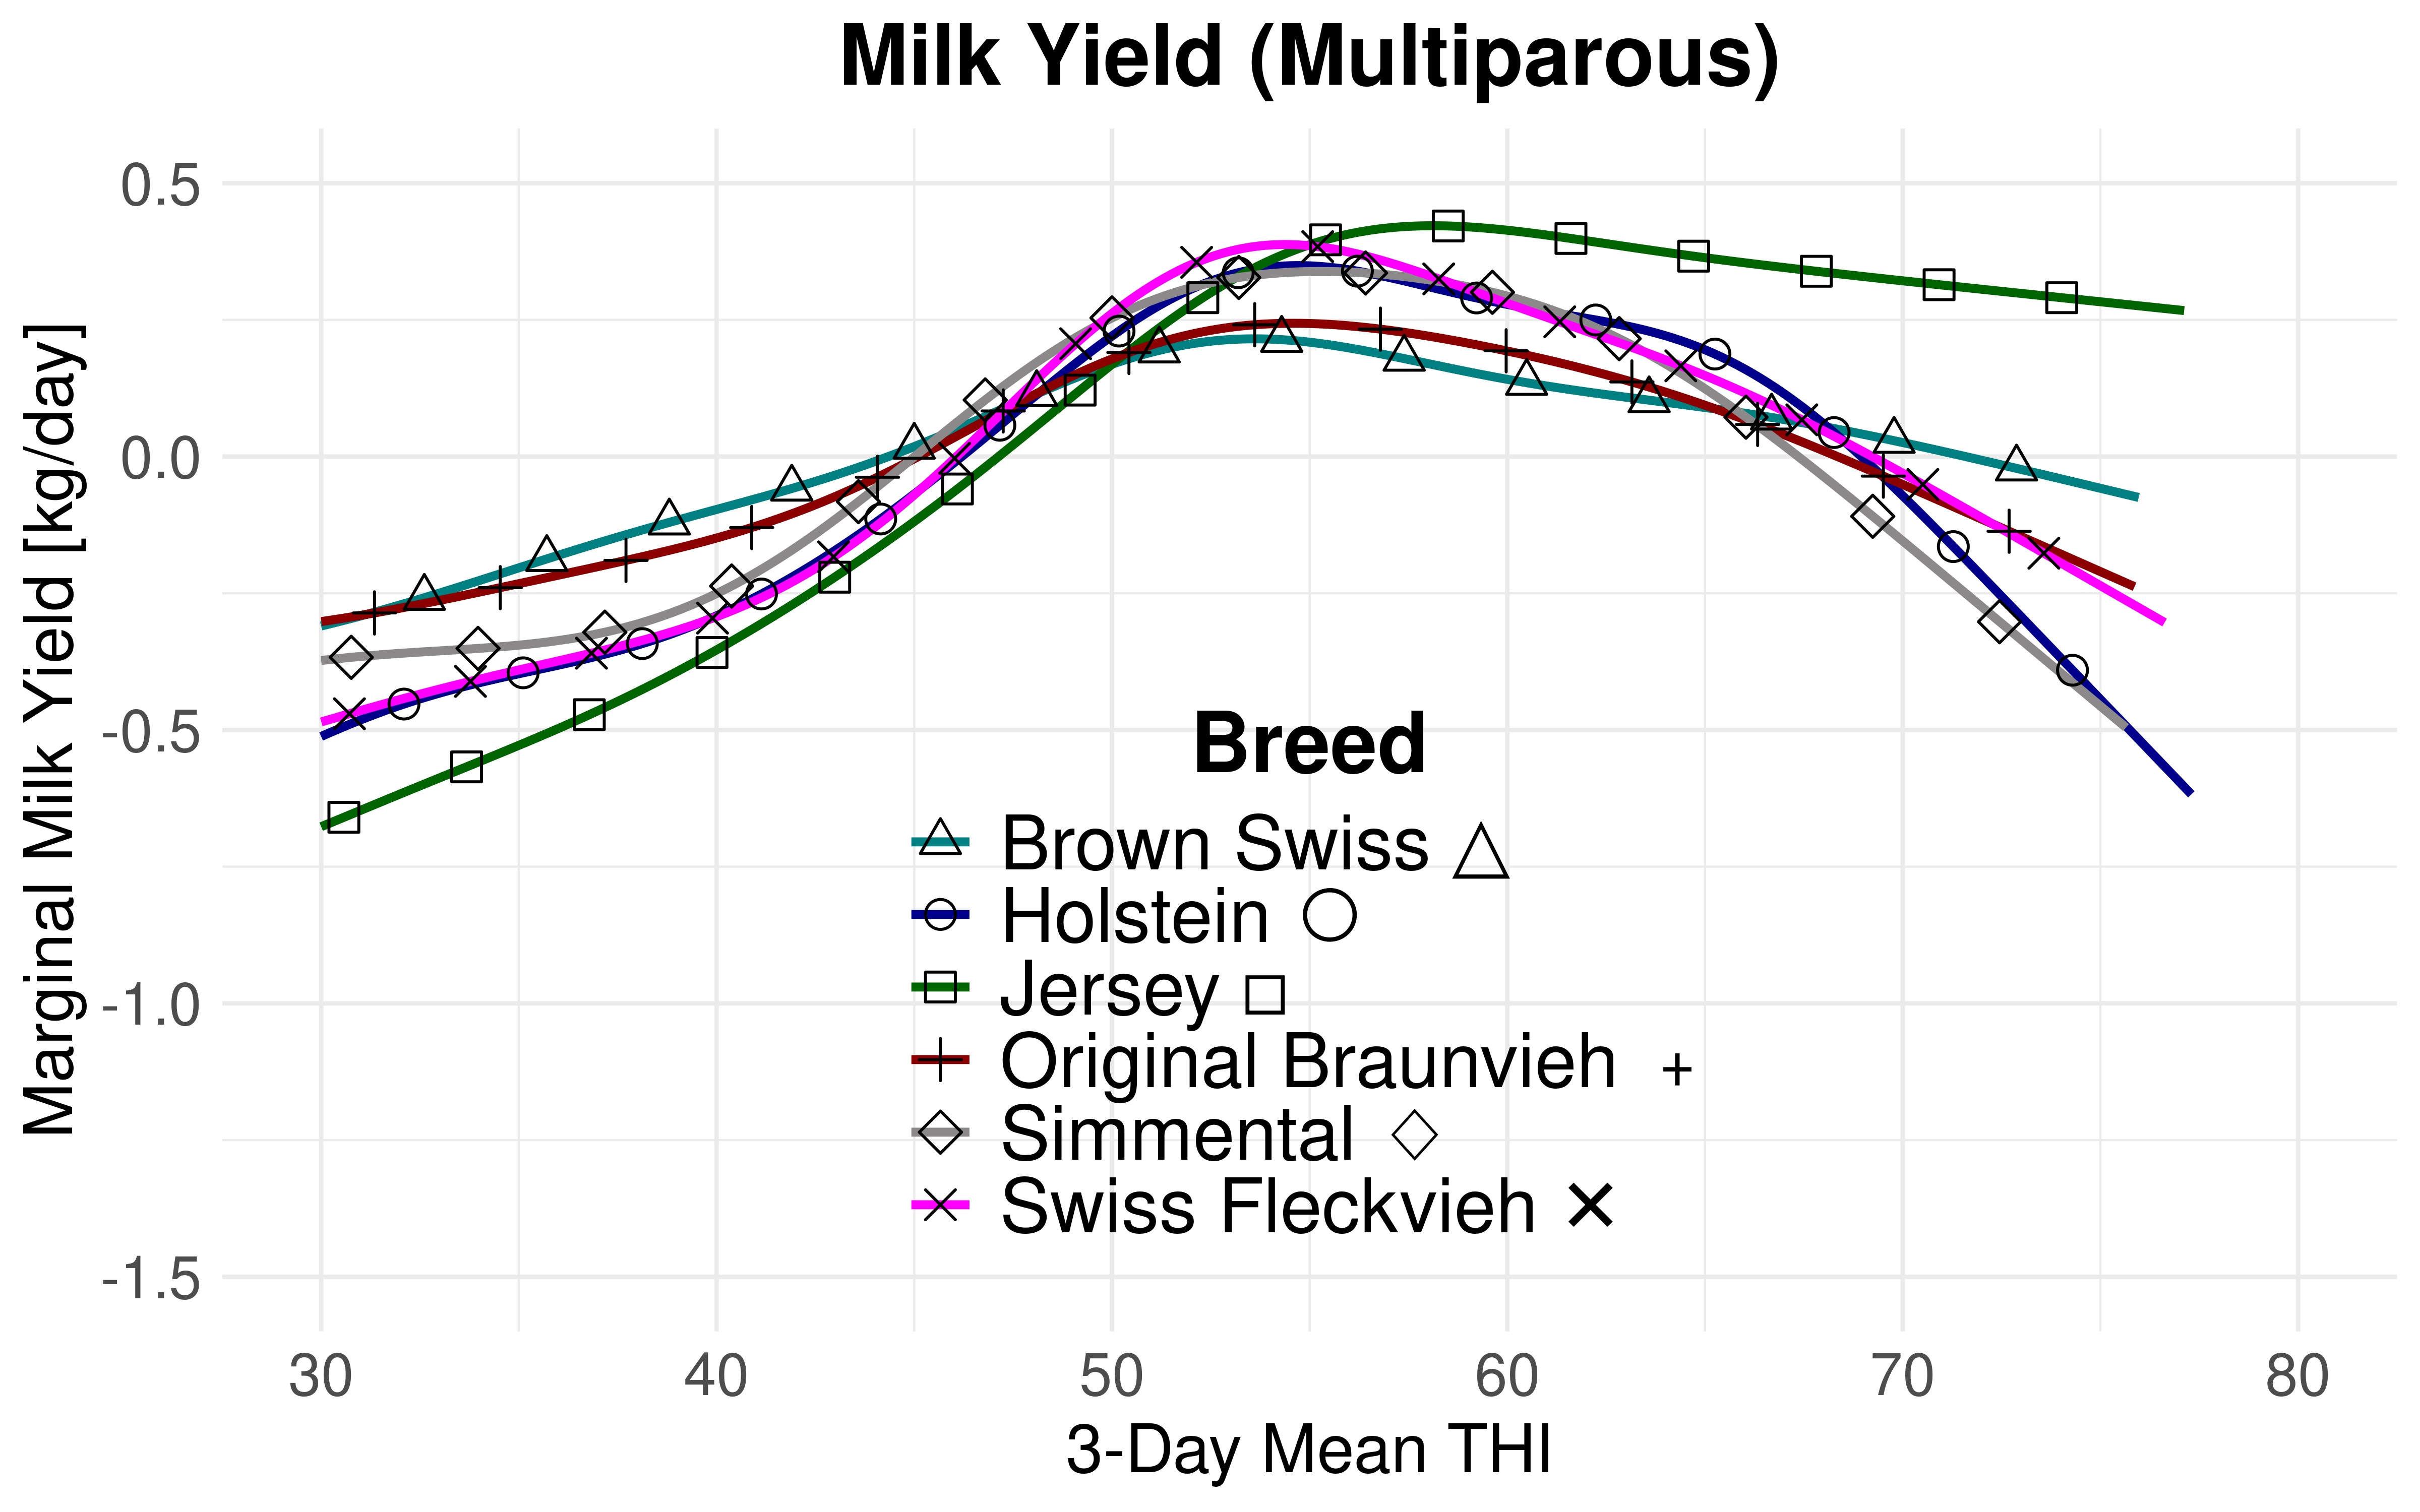
\includegraphics[width=\textwidth]{thesis/figures/results/milk_multiparous_overlapped.png}
        \caption{3-day mean marginal THI effect on milk yield multiparous Swiss dairy cows with data subsamples covering the full time period from 1982-2023.}
        \label{fig:milk_marginal_combined}
    \end{minipage}
    \hfill
    \begin{minipage}{0.49\textwidth}
        \centering
        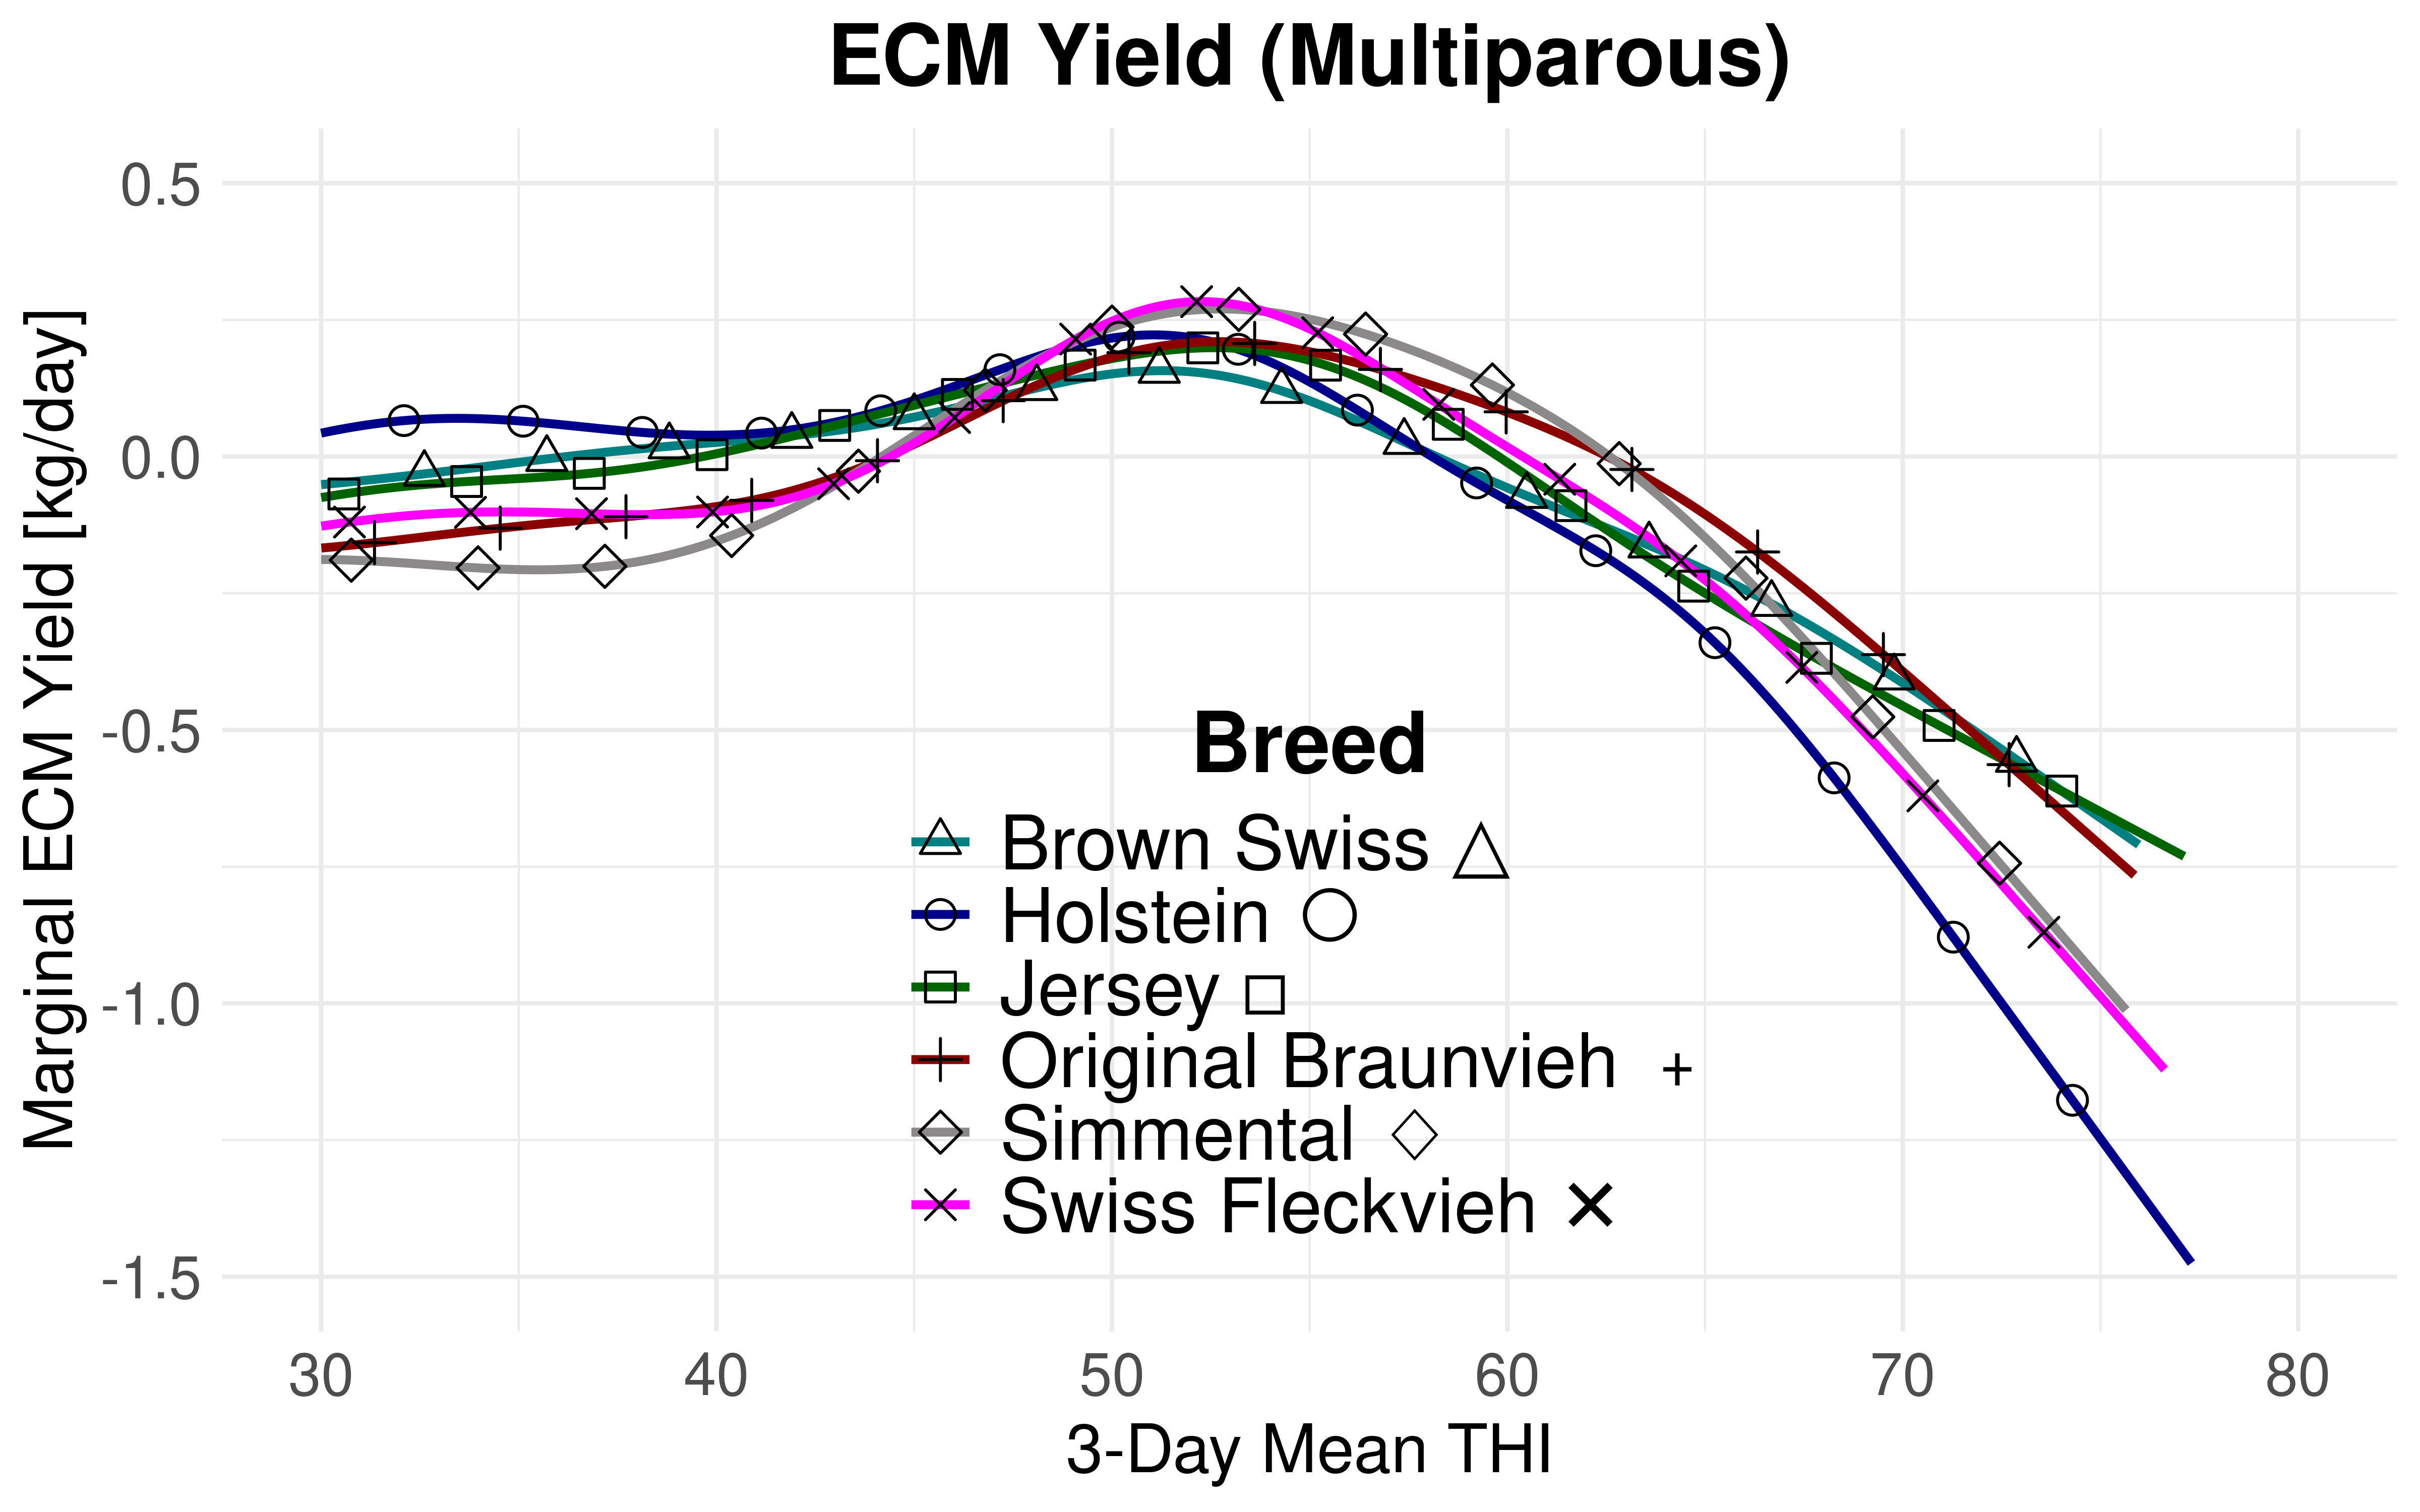
\includegraphics[width=\textwidth]{thesis/figures/results/ecm_multiparous_overlapped.png}
        \caption{3-day mean marginal THI effect on ECM yield multiparous Swiss dairy cows with data subsamples covering the full time period from 1982-2023.}
        \label{fig:ecm_marginal_combined}
    \end{minipage}
\end{figure}

The THI thresholds are lower for ECM yield compared to milk yield. Consequently, the milk component yields in relation to THI induce a leftward shift. Nonetheless, this shift does not remain uniform across all breeds. While the disparity between the lowest and highest THI turning points for milk yield is 4.56 for primiparous cows and 8.16 THI units for multiparous cows, the differences for ECM yield are notably smaller. Apparent benefits for certain breeds with respect to milk volume dissipate upon adjusting the milk volume for fat and protein yields. Figure~\ref{fig:milk_marginal_combined} and Figure~\ref{fig:ecm_marginal_combined} superpose the marginal effects of THI for each breed without confidence intervals to better illustrate this observation. The inverse relationship between THI and both fat and protein content is expected \citep{moore_how_2023}. \cite{vinet_estimation_2023} and \cite{hill_dairy_2015} have determined that declines in fat content in relation to THI manifest at an earlier stage or are stronger than protein declines. The specific individual contributions of protein and fat per breed to the observed shift and dissipation require further investigation.


\paragraph{Confidence Intervals}
The variability observed in the confidence intervals for each breed can be attributed to the employed subsampling strategy. The larger farms, the more samples per farm. Moreover, the available number of samples per farm also depends on the sampling strategy of the breeding associations. Table~\ref{table:milk_yield_subsample_stats_model_props} and Table~\ref{table:ecm_yield_subsample_stats_model_props} support this statement.  Consequently, our approach of incrementally incorporating farms into the dataset until a predetermined sample limit is reached results in a larger number of samples for these farms $t_s$. As a result, this approach contributes to diminished THI diversity, given that all samples gathered on a particular test-day at a given farm are associated with a single THI data point. This raises the question whether alternative subsampling methodologies at the farm level might need to be employed. Nonetheless, a careful interpretation of confidence intervals is necessary in this non-experimental study design and is further elaborated in Chapter~\ref{chap:conclusion}.

\paragraph{Split Period: Until 2010 - After 2010}
A striking difference emerges when splitting the data into two time periods: the THI turning points tend to be lower in the more recent data period from 2011 to 2023 compared to the period from 1982 to 2023. The Jersey breed poses an exception for ECM yield.

The average daily milk production is substantially higher today for all breeds relative to 13 years ago, attributed to successful breeding programs. The reduced THI turning points suggest that selective breeding has made dairy cows less tolerant to heat. The principal objectives of breeding are to enhance dairy performance with equivalent or relatively diminished input. Furthermore, long-term genetic selection exerts an influence on the metabolic system. The current selection strategies may prioritize enhancements in dairy performance without necessarily fostering heat resilience. As breeding continues to result in increased yields, offsetting heat-induced losses despite heightened heat exposure for dairy cows in Switzerland, this development potentially prompts more concerns regarding animal welfare rather than economic implications \citep{koenig_2023}. However, our results need further investigation with different cut-off years, multiple periods or different data subsampling strategies. Furthermore, shifts in THI turning points come along with changes in the loss rates. For example, simulations aggregating the daily effects with weather data over a long periods are necessary to further validate this negative change in heat-tolerance.